\documentclass[11pt,oneside,english]{book}

\usepackage{ifpdf}

\ifpdf
  \usepackage[pdftex]{graphicx}
  \pdfcompresslevel=9
  \DeclareGraphicsExtensions{.png,.jpg,.pdf,.mps}
\else
  \usepackage{graphicx}
  \DeclareGraphicsExtensions{.ps,.eps}
\fi
\usepackage[T1]{fontenc}
\usepackage[latin1]{inputenc}
\usepackage{geometry}
\geometry{verbose,letterpaper,tmargin=1in,bmargin=1in,lmargin=1in,rmargin=1in}
\usepackage{babel}
\setcounter{secnumdepth}{3}
\setlength\parskip{\medskipamount}
\setlength\parindent{0pt}
\usepackage{url}
\usepackage{pslatex}
\usepackage[colorlinks=false]{hyperref}

\newcommand{\Erlang}            % Write Erlang correctly
        {{\sc Erlang}}


\newcommand{\Yaws}            % Write Yaws correctly
        {{\sc Yaws}}


\makeatletter

\usepackage[T1]{fontenc}
\usepackage{xspace}
%\usepackage{html}

\makeatother
\begin{document}



\title{Yaws - Yet Another Web Server}


\author{Claes Wikstrom\\
klacke@hyber.org}





\maketitle
\tableofcontents{}



\chapter{Introduction}


\begin{figure}[h]
\begin{center}

 
\includegraphics[scale=0.6] {yaws_head}

\end{center}
\end{figure}

\Yaws\  is an \Erlang\  web server. It's written in \Erlang\  and it uses
\Erlang\  as its embedded language similar to PHP in Apache or Java in Tomcat.

The advantages of \Erlang\  as an embedded web page language as opposed to
Java or PHP are many.
\begin{itemize}

\item{Speed - Using \Erlang\  for both implementing the web server itself as well
as embedded script language gives excellent dynamic page generation
performance.}

\item{Beauty - Well this is subjective}

\item{Scalability - due to the lightweight processes of \Erlang{}, \Yaws\
is able to handle a very large number of concurrent connections}

\end{itemize}

\Yaws\  has a wide feature set; it supports:

\begin{itemize}
\item HTTP 1.0 and HTTP 1.1
\item Static content page delivery
\item Dynamic content generation using embedded \Erlang\  code in the
HTML pages
\item NCSA combined/XLF/ELF log format traffic logs
\item Virtual hosting with several servers on the same IP address
\item Multiple servers on multiple IP addresses
\item HTTP tracing for debugging
\item An interactive interpreter environment in the Web server for use while
developing and debugging a web site
\item RAM caching of commonly accessed pages
\item Full streaming capabilities of both upload and download of dynamically
generated pages
\item SSL
\item Support for WWW-Authenticated pages
\item Support API for cookie based sessions
\item Application Modules where virtual directory hierarchies can
be made
\item Embedded mode
\item WebSockets (RFC 6455)
\item Long polling (COMET) applications
\item Forward and reverse proxying
\end{itemize}

\section{Prerequisites}
This document requires that the reader:
\begin{itemize}
\item Is well acquainted with the \Erlang\  programming language.
\item Understands basic Web technologies.
\end{itemize}


\section{A tiny example}

We introduce \Yaws\  by help of a tiny example.
 The web server \Yaws\  serves  and delivers
static content pages similar to any old web server, except that \Yaws\  does this
much faster than most web servers. It's the dynamic pages
that makes \Yaws\  interesting. Any page with the suffix ``.yaws'' is considered
a dynamic \Yaws\  page. A \Yaws\  page can contain embedded \Erlang\  snippets that
are executed while the page is being delivered to the WWW browser.

Example 1.1 is the HTML code for a small \Yaws\  page.


\begin{figure}[h]
\begin{verbatim}
<html>

<p> First paragraph

<erl>
out(Arg) ->
    {html, "<p>This string gets inserted into HTML document dynamically"}.
</erl>

<p> And here is some more HTML code

</html>
\end{verbatim}
\caption{Example 1.1}
\end{figure}

It illustrates the basic idea behind \Yaws{}. The HTML code, generally
stored in a file ending with a ``.yaws'' suffix, can contain
\verb+<erl>+ and \verb+</erl>+ tags and inside these tags an
\Erlang\ function called \verb+out/1+ gets called and the output of
that function is inserted into the HTML document, dynamically.

It is possible to have several chunks of HTML code together with several
chunks of \Erlang\  code in the same \Yaws\  page.

The \verb+Arg+ argument supplied to the automatically invoked \verb+out/1+
function is an \Erlang\  record that contains various data which is interesting
when generating dynamic pages. For example the HTTP headers which were sent
from the WWW client, the actual TCP/IP socket leading to the WWW client.
This will be elaborated on thoroughly in later chapters.

The \verb+out/1+ function returned the tuple \verb+{html, String}+ and
\verb+String+ gets inserted into the HTML output. There are number
of different return values that can be returned from the \verb+out/1+ function
in order to control the behavior and output from the \Yaws\  web server.


\chapter{Compile, Install, Config and Run}

This chapter is more of a ``Getting started'' guide than a full
description of the \Yaws\ configuration.  \Yaws\ is hosted on Github
at \url{ https://github.com/klacke/yaws }. This is where the source
code resides in a git repository and the latest unreleased version is
available via git through the following commands:

\begin{verbatim}

$ git clone https://github.com/klacke/yaws

\end{verbatim}

Released version of \Yaws\ are available at
\url{http://yaws.hyber.org/download}.

\subsection{Compile and Install}

To compile and install a \Yaws\  release
one of the prerequisites is a properly installed \Erlang\  system. \Yaws\
runs on \Erlang\/OTP releases R16B01 and newer. Get \Erlang\  from
\url{http://www.erlang.org/}

Compile and install is straight forward:
\begin{verbatim}
# cd /usr/local/src
# tar xfz yaws-X.XX.tar.gz
# cd yaws-X.XX
# ./configure && make
# make install
\end{verbatim}

The \verb+make+ command will compile the \Yaws\  web server with the
\verb+erlc+ compiler found by the configure script.

\begin{itemize}

\item  \verb+make install+ - will install the executable called
         \verb+yaws+ in \verb+/usr/local/bin/+ and a working
         configuration file in \verb+/usr/local/etc/yaws.conf+

\end{itemize}

Alternatively, you can compile \Yaws\  with \verb+rebar+ as follows:

\begin{verbatim}
# rebar get-deps compile
\end{verbatim}

If you want to build with SOAP support, run the following command:

\begin{verbatim}
# YAWS_SOAP=1 rebar get-deps compile
\end{verbatim}

To create a \Yaws\  release with \verb+reltool+, execute the following
command:

\begin{verbatim}
# rebar generate
\end{verbatim}

Because it bundles Erlang/OTP and all of the application's dependencies,
the generated release found in \verb+rel/+ is standalone and has no
external requirements. A future release of \verb+rebar+ will allow you
to create a slim release that doesn't bundle Erlang/OTP. This is not yet
available.

While developing a \Yaws\ site, it's typically most convenient to do a
\verb+local+ install and run \Yaws\ as a non-privileged user using
\verb+--prefix+ option of the \verb+configure+ script:
\begin{verbatim}
# ./configure --prefix=/path/to/yaws && make install
# /path/to/yaws/bin/yaws -i
\end{verbatim}

\subsection{Configure}
Let's take a look at the config file that gets written after a \verb+local+
install in \verb+/home/klacke/yaws/+. The file is
\verb+/home/klacke/yaws/etc/yaws/yaws.conf+:


\begin{figure}[h]
\begin{verbatim}

# first we have a set of globals

logdir = /home/klacke/yaws/var/log/yaws
ebin_dir = /home/klacke/yaws/lib/yaws/examples/ebin
include_dir = /home/klacke/yaws/lib/yaws/examples/include

...

# and then a set of servers

<server localhost>
        port = 8000
        listen = 127.0.0.1
        docroot = /home/klacke/yaws/var/yaws/www
</server>


\end{verbatim}
\caption{Minimal Local Configuration}
\end{figure}

The configuration consists of an initial set of global
variables that are valid for all defined servers.

The only global directive we need to care about for now is the logdir.
\Yaws\ produces a number of log files. We start \Yaws\ interactively as

\begin{verbatim}
# ~/bin/yaws -i
Erlang (BEAM) emulator version 5.1.2.b2 [source]

Eshell V5.1.2.b2  (abort with ^G)
1>
=INFO REPORT==== 30-Oct-2002::01:38:22 ===
Using config file /home/klacke/yaws/etc/yaws/yaws.conf
=INFO REPORT==== 30-Oct-2002::01:38:22 ===
Listening to 127.0.0.1:8000 for servers ["localhost:8000"]

1>
\end{verbatim}

By starting \Yaws\ in interactive mode (using the command switch
\textit{-i}) we get a regular \Erlang\ prompt. This is most convenient
when developing \Yaws\ pages. For example we:

\begin{itemize}
\item{Can dynamically compile and load optional helper modules we need.}
\item{Get all the crash and error reports written directly to the
terminal.}
\end{itemize}

The configuration in Example 2.1 defined one HTTP server on address
127.0.0.1:8000 called "localhost".  It is important to understand the
difference between the name and the address of a server. The name is
the expected value in the client HTTP \verb+Host:+ header. That is
typically the same as the fully-qualified DNS name of the server
whereas the address is the actual IP address of the server.

Since \Yaws\  supports virtual hosting with several servers on the same
IP address, this matters.

Nevertheless, our server listens to \textit{127.0.0.1:8000} and
has the name "localhost", thus the correct URL for this server
is \verb+http://localhost:8000+.

The document root (docroot) for the server is a copy of the \verb+www+ directory
in the \Yaws\ source code distribution. This directory contains a bunch of
examples and we should be able to run all those example now on the URL
\verb+http://localhost:8000+.

Instead of editing and adding files in the \Yaws\ \verb+www+
directory, we create yet another server on the same IP address but a
different port number --- and in particular a different document root
where we can add our own files.

\begin{verbatim}
# mkdir ~/test
# mkdir ~/test/logs
\end{verbatim}

Now change the config so it looks like this:

\begin{verbatim}

logdir = /home/klacke/test/logs
ebin_dir = /home/klacke/test
include_dir = /home/klacke/test

<server localhost>
        port = 8000
        listen = 127.0.0.1
        docroot = /home/klacke/yaws/var/yaws/www
</server>

<server localhost>
        port = 8001
        listen = 127.0.0.1
        docroot = /home/klacke/test
</server>


\end{verbatim}

We define two servers, one being the original default
and a new pointing to a document root in our home directory.

We can now start to add static content in the form of HTML pages,
dynamic content in the form of \verb+.yaws+ pages or
\Erlang\ \verb+.beam+ code that can be used to generate the dynamic
content.

The load path will be set so that beam code in the directory
\char`\~\verb+/test+ will be automatically loaded when referenced.

It is best to run \Yaws\  interactively while developing the site.
In order to start the \Yaws\  as a daemon, we give the flags:
\begin{verbatim}
# yaws -D --heart
\end{verbatim}

The \textit{-D} or \textit{--daemon} flags instructs \Yaws\ to run as
a daemon and the \textit{--heart} flag will start a heartbeat program
called heart which restarts the daemon if it should crash or if it
stops responding to a regular heartbeat. By default, heart will
restart the daemon unless it has already restarted 5 times in 60
seconds or less, in which case it considers the situation fatal and
refuses to restart the daemon again. The \textit{-heart-restart=C,T}
flag changes the default 5 restarts in 60 seconds to \textit{C}
restarts in \textit{T} seconds. For infinite restarts, set both
\textit{C} and \textit{T} to 0. This flag also enables the
\textit{--heart} flag.

Once started in daemon mode, we have very limited ways of interacting
with the daemon. It is possible to query the daemon using:
\begin{verbatim}
# yaws -S
\end{verbatim}

This command produces a simple printout of uptime and number of hits
for each configured server.

If we change the configuration, we can HUP the daemon using the
command:
\begin{verbatim}
# yaws -h
\end{verbatim}

This will force the daemon to reread the configuration file.



\chapter{Static content}

\Yaws\  acts very much like any regular web server while delivering
static pages. By default \Yaws\  will cache static content in RAM.
The caching behavior is controlled by a number of global
configuration directives. Since the RAM caching occupies memory,
it may be interesting to tweak the default values for the caching directives
or even to turn it off completely.

The following configuration directives control the caching behavior
\begin{itemize}
\item \textit{max\_num\_cached\_files = Integer}

\Yaws\   will  cache  small  files  such  as  commonly
              accessed  GIF images in RAM.  This directive sets a
              maximum number on the number of cached files.   The
              default value is 400.

\item\textit{max\_num\_cached\_bytes = Integer}

 This  directive  controls  the  total amount of RAM
             which can maximally be used for cached  RAM  files.
              The default value is 1000000, 1 megabyte.


\item\textit{max\_size\_cached\_file = Integer}

 This  directive  sets  a  maximum size on the files
              that are RAM cached by \Yaws{}.  The default value is
              8000 bytes, 8 batters.



\end{itemize}

It may be considered to be confusing, but the numbers specified
in the above mentioned cache directives are local to each
server. Thus if we have specified \verb+max_num_cached_bytes = 1000000+
and have defined 3 servers, we may actually use $3 * 1000000$ bytes.




\chapter{Dynamic content}

Dynamic content is what \Yaws\ is all about. Most web servers are
designed with HTTP and static content in mind whereas \Yaws\ is
designed for dynamic pages from the start.  Most large sites on the
Web today make heavy use of dynamic pages.


\section{Introduction}

When the client \verb+GET+s a page that has a ``.yaws'' suffix, the
\Yaws\ server will read that page from the hard disk and divide it in
parts that consist of HTML code and \Erlang\ code. Each chunk of
\Erlang\ code will be compiled into a module. The chunk of
\Erlang\ code must contain a function \verb+out/1+. If it doesn't the
\Yaws\ server will insert a proper error message into the generated
HTML output.

When the \Yaws\ server ships a \verb+.yaws+ page it will process it
chunk by chunk through the \verb+.yaws+ file. If it is HTML code, the
server will ship that as is, whereas if it is \Erlang\ code, the
\Yaws\ server will invoke the \verb+out/1+ function in that code and
insert the output of that \verb+out/1+ function into the stream of
HTML that is being shipped to the client.

\Yaws\ will (of course) cache the result of the compilation and the
next time a client requests the same \verb+.yaws+ page \Yaws\ will be
able to invoke the already-compiled modules directly.


\section{EHTML}

There are two ways to make the \verb+out/1+ function generate HTML
output. The first and most easy to understand is by returning a tuple
\verb+{html, String}+ where \verb+String+ then is regular HTML data
(possibly as a deep list of strings and/or binaries) which will simply
be inserted into the output stream.
An example:

\begin{verbatim}
<html>
<h1> Example 1 </h1>

<erl>
out(A) ->
    Headers = A#arg.headers,
    {html, io_lib:format("You say that you're running ~p",
                         [Headers#headers.user_agent])}.

</erl>

</html>

\end{verbatim}


The second way to generate output is by returning a tuple
\verb+{ehtml, EHTML}+ or \verb+{exhtml, EHTML}+. The exhtml variant
generates strict XHTML code. The term \verb+EHTML+ must adhere to the
following structure:

$EHTML = [EHTML] | \{TAG, Attrs, Body\} |
               \{TAG, Attrs\} | \{TAG\} |\\*
\hspace*{0.75 in} \{Module, Fun, [Args]\} | fun/0 |\\*
\hspace*{0.75 in} binary() | character()$

$TAG   = atom()$

$Attrs = [\{HtmlAttribute, Value\}]$

$HtmlAttribute = atom()$

$Value = string() | binary() | atom() | integer() | float() |\\*
\hspace*{0.55 in} \{Module, Fun, [Args]\} | fun/0$

$Body  = EHTML$

We give an example to show what we mean. The tuple

\begin{verbatim}
{ehtml, {table, [{bgcolor, grey}],
         [
          {tr, [],
           [
            {td, [], "1"},
            {td, [], "2"},
            {td, [], "3"}
           ]
          },
          {tr, [],
           [{td, [{colspan, "3"}], "444"}]}]}}.
\end{verbatim}

expands into the following HTML code:

\begin{verbatim}
<table bgcolor="grey">
  <tr>
    <td> 1 </td
    <td> 2 </td>
    <td> 3 </td>
  </tr>
  <tr>
    <td colspan="3"> 444 </td>
  </tr>
</table>

\end{verbatim}

At a first glance it may appears as if the HTML code is more beautiful
than the \Erlang\ tuple. That may very well be the case from a purely
aesthetic point of view. However the \Erlang\ code has the advantage
of being perfectly indented by editors that have syntax support for
\Erlang\ (read Emacs). Furthermore, the \Erlang\ code is easier to
manipulate from an \Erlang\ program.

Note that ehtml supports function calls as values. Functions can
return any legal ehtml value, including other function
values. \Yaws\ supports \verb+{M,F,[Args]}+ and \verb+fun/0+ function
value forms.

As an example of some more interesting ehtml we could have an
\verb+out/1+ function that prints some of the HTTP headers.  In the
\verb+www+ directory of the \Yaws\ source code distribution we have a
file called \verb+arg.yaws+. The file demonstrates the \verb+Arg+
\verb+#arg+ record parameter which is passed to the \verb+out/1+
function.

But before we discuss that code, we describe the \verb+Arg+ record
in detail.

Here is the \verb+yaws_api.hrl+ file which is in included by default
in all \Yaws\ files. The \verb+#arg{}+ record contains many fields
that are useful when processing HTTP request dynamically.  We have
access to basically all the information associated with the client
request such as:

\begin{itemize}

\item The actual socket leading back to the HTTP client
\item All the HTTP headers -- parsed into a \verb+#headers+ record
\item The HTTP request -- parsed into a \verb+#http_request+ record
\item \verb+clidata+ -- data which is \verb+POST+ed by the client
\item \verb+querydata+ -- this is the remainder of the URL following
  the first occurrence of a '?' character, if any.
\item \verb+docroot+ -- the absolute path to the docroot of the
  virtual server that is processing the request.
\end{itemize}



\begin{verbatim}


-record(arg, {
          clisock,        % the socket leading to the peer client
          client_ip_port, % {ClientIp, ClientPort} tuple
          headers,        % headers
          req,            % request
          orig_req,       % original request
          clidata,        % The client data (as a binary in POST requests)
          server_path,    % The normalized server path
                          % (pre-querystring part of URI)
          querydata,      % For URIs of the form ...?querydata
                          %  equiv of cgi QUERY_STRING
          appmoddata,     % (deprecated - use pathinfo instead) the remainder
                          % of the path leading up to the query
          docroot,        % Physical base location of data for this request
          docroot_mount,  % virtual directory e.g /myapp/ that the docroot
                          %  refers to.
          fullpath,       % full deep path to yaws file
          cont,           % Continuation for chunked multipart uploads
          state,          % State for use by users of the out/1 callback
          pid,            % pid of the yaws worker process
          opaque,         % useful to pass static data
          appmod_prepath, % (deprecated - use prepath instead) path in front
                          %  of: <appmod><appmoddata>
          prepath,        % Path prior to 'dynamic' segment of URI.
                          %  ie http://some.host/<prepath>/<script-point>/d/e
                          % where <script-point> is an appmod mount point,
                          % or .yaws,.php,.cgi,.fcgi etc script file.
          pathinfo        % Set to '/d/e' when calling c.yaws for the request
                          % http://some.host/a/b/c.yaws/d/e
                          %  equiv of cgi PATH_INFO
         }).

-record(http_request, {method,
                       path,
                       version}).


-record(headers, {
          connection,
          accept,
          host,
          if_modified_since,
          if_match,
          if_none_match,
          if_range,
          if_unmodified_since,
          range,
          referer,
          user_agent,
          accept_ranges,
          cookie = [],
          keep_alive,
          location,
          content_length,
          content_type,
          content_encoding,
          authorization,
          transfer_encoding,
          x_forwarded_for,
          other = []   % misc other headers
         }).

\end{verbatim}


There are a number of \textit{advanced} fields in the \verb+#arg+
record such as \verb+appmod+ and \verb+opaque+ that will be discussed
in later chapters.

Now, we show some code which displays the content of the \verb+Arg+
\verb+#arg+ record.  The code is available in \verb+yaws/www/arg.yaws+
and after a \verb+local_install+ a request to
\url{http://localhost:8000/arg.yaws} will run the code.

\begin{verbatim}

<html>

<h2> The Arg </h2>

<p>This page displays the Arg #argument structure
supplied to the out/1 function.

<erl>


out(A) ->
    Req = A#arg.req,
    H = yaws_api:reformat_header(A#arg.headers),
    {ehtml,
     [{h4,[], "The headers passed to us were:"},
      {hr},
      {ol, [],lists:map(fun(S) -> {li,[], {p,[],S}} end,H)},

      {h4, [], "The request"},
      {ul,[],
       [{li,[], f("method: ~s",  [Req#http_request.method])},
        {li,[], f("path: ~p",    [Req#http_request.path])},
        {li,[], f("version: ~p", [Req#http_request.version])}]},

      {hr},
      {h4, [], "Other items"},
      {ul,[],
       [{li,[], f("clisock from: ~p", [inet:peername(A#arg.clisock)])},
        {li,[], f("docroot: ~s",      [A#arg.docroot])},
        {li,[], f("fullpath: ~s",     [A#arg.fullpath])}]},
      {hr},
      {h4, [], "Parsed query data"},
      {pre,[], f("~p", [yaws_api:parse_query(A)])},
      {hr},
      {h4,[], "Parsed POST data "},
      {pre,[],  f("~p", [yaws_api:parse_post(A)])}]}.

</erl>

</html>

\end{verbatim}

The code utilizes four functions from the \verb+yaws_api+ module.  The
\verb+yaws_api+ module is a general purpose www API module that
contains various functions that are handy while developing
\Yaws\ code. We will see many more of those functions during the
examples in the following chapters.

The functions used are:

\begin{itemize}
\item \verb+yaws_api:f/2+ --- alias for \verb+io_lib:format/2+. The
  \verb+f/2+ function is automatically \verb+-included+ in all
  \Yaws\ code.
\item \verb+yaws_api:reformat_header/1+ --- This function takes the
  \#headers record and unparses it, that is reproduces regular text.
\item \verb+yaws_api:parse_query/1+ --- The topic of the next section.
\item \verb+yaws_api:parse_post/1+ --- Ditto.
\end{itemize}


\section{POSTs}

\subsection{Queries}

The user can supply data to the server in many ways. The most
common is to give the data in the actual URL.
If we invoke:

\verb+GET http://localhost:8000/arg.yaws?kalle=duck&goofy=unknown+

we pass two parameters to the \verb+arg.yaws+ page.  That data is
URL-encoded by the browser and the server can retrieve the data by
looking at the remainder of the URL following the '?' character.  If
we invoke the \verb+arg.yaws+ page with the above mentioned URL we get
as the result of \verb+yaws_api:parse_query/1+:

$kalle = duck$

$goofy = unknown$

In \Erlang\  terminology, the call \verb+yaws_api:parse_query(Arg)+ returns
the list:
\begin{verbatim}
[{"kalle", "duck"}, {"goofy", "unknown"}]
\end{verbatim}

Both the key and the value are strings. Hence, a web page can contain URLs with
a query and thus pass data to the web server. This scheme works with any kind of
requests. It is the easiest way to pass data to the Web server since no form is
required in the web page.


\subsection{Forms}

In order to \verb+POST+ data a form is required. Say that we have a
page called \verb+form.yaws+ that contain the following code:

\begin{verbatim}
<html>
<form action="/post_form.yaws"
      method="post"

<p> A Input field
<input name="xyz" type="text">
<input type="submit">
</form>
</html>
\end{verbatim}

This will produce a page with a simple input field and a submit button.

\begin{figure}[h]
\begin{center}

 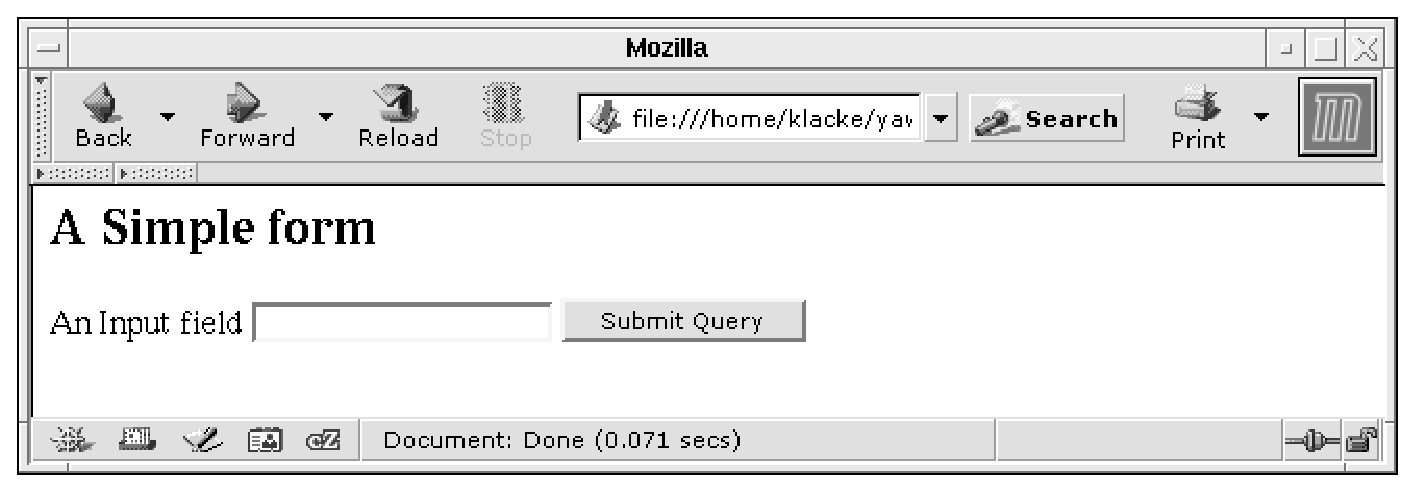
\includegraphics[scale=0.6] {a}

\end{center}
\end{figure}


If we enter something---say, ``Hello there''---in the input field and
click the submit button the client will request the page indicated in
the ``action'' attribute, namely \verb+post_form.yaws+.

If that \Yaws\  page has the following code:

\begin{verbatim}
out(A) ->
   L = yaws_api:parse_post(A),
   {html, f("~p", [L])}
\end{verbatim}

The user will see the output

\begin{verbatim}
[{"xyz", "Hello there"}]
\end{verbatim}

The differences between using the query part of the URL
and a form are the following:

\begin{itemize}
\item Using the query arg works with any kind of requests. We parse the query
  argument with the function \verb+yaws_api:parse_query(Arg)+

\item If we use a form and \verb+POST+ the user data the client will
  transmit the user data in the body of the request.  That is, the
  client sends a request to get the page using the \verb+POST+ method
  and it then attaches the user data---encoded---into the body of the
  request.

A \verb+POST+ request can have a query part in its URL as well as user
data in the body.
\end{itemize}


\section{POSTing files}

It is possible to upload files from the client to the server by means
of \verb+POST+. We indicate this in the form by telling the browser
that we want a different encoding. Here is an example form that does
this:
\begin{verbatim}

out(A) ->
    Form =
        {form, [{enctype, "multipart/form-data"},
                {method, post},
                {action, "file_upload_form.yaws"}],
                [{input, [{type, submit}, {value, "Upload"}]},
                 {input, [{type,file}, {width, "50"}, {name, foo}]}]},
    {ehtml, {html,[], [{h2,[], "A simple file upload page"},
                      Form]}}.

\end{verbatim}

As shown in the figure, the page delivers the entire HTML page with
enclosing \verb+html+ markers.


\begin{figure}[h]
\begin{center}

 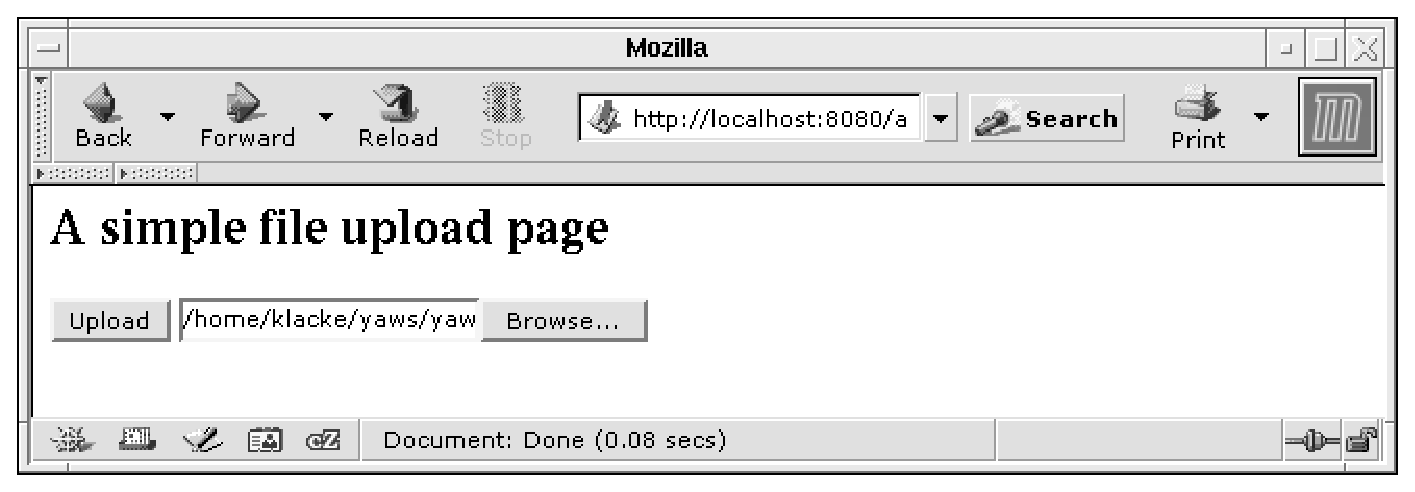
\includegraphics[scale=0.6] {b}

\end{center}
\end{figure}

The user gets an option to browse the local host for a file
or the user can explicitly fill in the file name in the input
field. The file browsing part is automatically taken care of by the
browser.

The action field in the form states that the client shall POST to a
page called \verb+file_upload_form.yaws+. This page will get the
contents of the file in the body of the \verb+POST+ message. To read
it, we use the \verb+yaws_multipart+ module, which provides the
following capabilities:

\begin{enumerate}
\item It reads all parameters --- files uploaded and other simple
  parameters.
\item It takes a few options to help file uploads. Specifically:
\begin{enumerate}
\item \verb+{max_file_size, MaxBytes}+: if the file size in bytes
  exceeds \verb+MaxBytes+, return an error
\item \verb+no_temp_file+: read the uploaded file into memory without
  any temp files
\item \verb+{temp_file,FullFilePath}+: specify \verb+FullFilePath+ for
  the temp file; if not given, a unique file name is generated
\item \verb+{temp_dir, TempDir}+: specify \verb+TempDir+ as the
  directory to store the uploaded temp file; if this option is not
  provided, then by default an OS-specific temp directory such as
  \verb+/tmp+ is used
\item \verb+list+: return file data in list form; this is the default
\item \verb+binary+: return file data in binary form
\end{enumerate}
\end{enumerate}

Note that the \verb+list+ and \verb+binary+ options affect only file
data, not filenames, headers, or other parameters associated with each
file. These are always returned as strings.

Just call \verb+yaws_multipart:read_multipart_form+ from your
\verb+out/1+ function and it'll return a tuple with the first element
set to one of these three atoms:

\begin{itemize}
\item \verb+get_more+: more data needs to be read; return this tuple
  directly to \Yaws\ from your \verb+out/1+ function and it will call
  your \verb+out/1+ function again when it has read more \verb+POST+
  data, at which point you must call \verb+read_multipart_form+ again
\item \verb+done+: multipart form reading is complete; a
  \verb+dict+ full of parameters is returned
\item \verb+error+: an error occurred
\end{itemize}

The \verb+dict+ returned with \verb+done+ allows you to query it for
parameters by name. For file upload parameters, it returns one of the
following lists:

\begin{verbatim}
[{filename, "name of the uploaded file as entered on the form"},
 {value, Contents_of_the_file_all_in_memory} | _T]
\end{verbatim}

or:

\begin{verbatim}
[{filename, "name of the uploaded file as entered on the form"},
 {temp_file, "full pathname of the temp file"} | _T]
\end{verbatim}

Some multipart/form messages also headers such as \verb+Content-Type+
and \verb+Content-Transfer-Encoding+ for different subparts of the
message. If these headers are present in any subpart of a
multipart/form message, they're also included in that subpart's
parameter list, like this:

\begin{verbatim}
[{filename, "name of the uploaded file as entered on the form"},
 {value, Contents_of_the_file_all_in_memory},
 {content_type, "image/png"} | _T]
\end{verbatim}

Note that for the temporary file case, it's your responsibility to
delete the file when you're done with it.

Here's an example:

\begin{verbatim}
-module(my_yaws_controller).
-export([out/1]).

out(Arg) ->
    Options = [no_temp_file],
    case yaws_multipart:read_multipart_form(Arg, Options) of
        {done, Params} ->
            io:format("Params : ~p~n", [Params]),
            {ok, [{filename, FileName},{value,FileContent}|_]} =
                dict:find("my_file", Params),
            AnotherParam = dict:find("another_param", Params);
        %% do something with FileName, FileContent and AnotherParam
        {error, Reason} ->
            io:format("Error reading multipart form: ~s~n", [Reason]);
        Other -> Other
    end.
\end{verbatim}

Here, \verb+my_yaws_controller+ is a user-defined module compiled as
usual with \verb+erlc+ with the resulting \verb+.beam+ file placed in
the \Yaws\ load path. The module is then registered with \Yaws\ as an
\emph{appmod} to allow it to receive and process requests---see
section \ref{appmods} for more details.

\chapter{Mode of operation}

\section{On-the-fly compilation}
When the client requests a \Yaws\ page, \Yaws\ will look in its caches
(there is one cache per virtual server) to see if it finds the
requested page in the cache. If \Yaws\ doesn't find the page in the
cache, it will compile the page. This only happens the first time a
page is requested.  Say that the page is 400 bytes big and has the
following layout:


\begin{figure}[h]
\begin{center}

 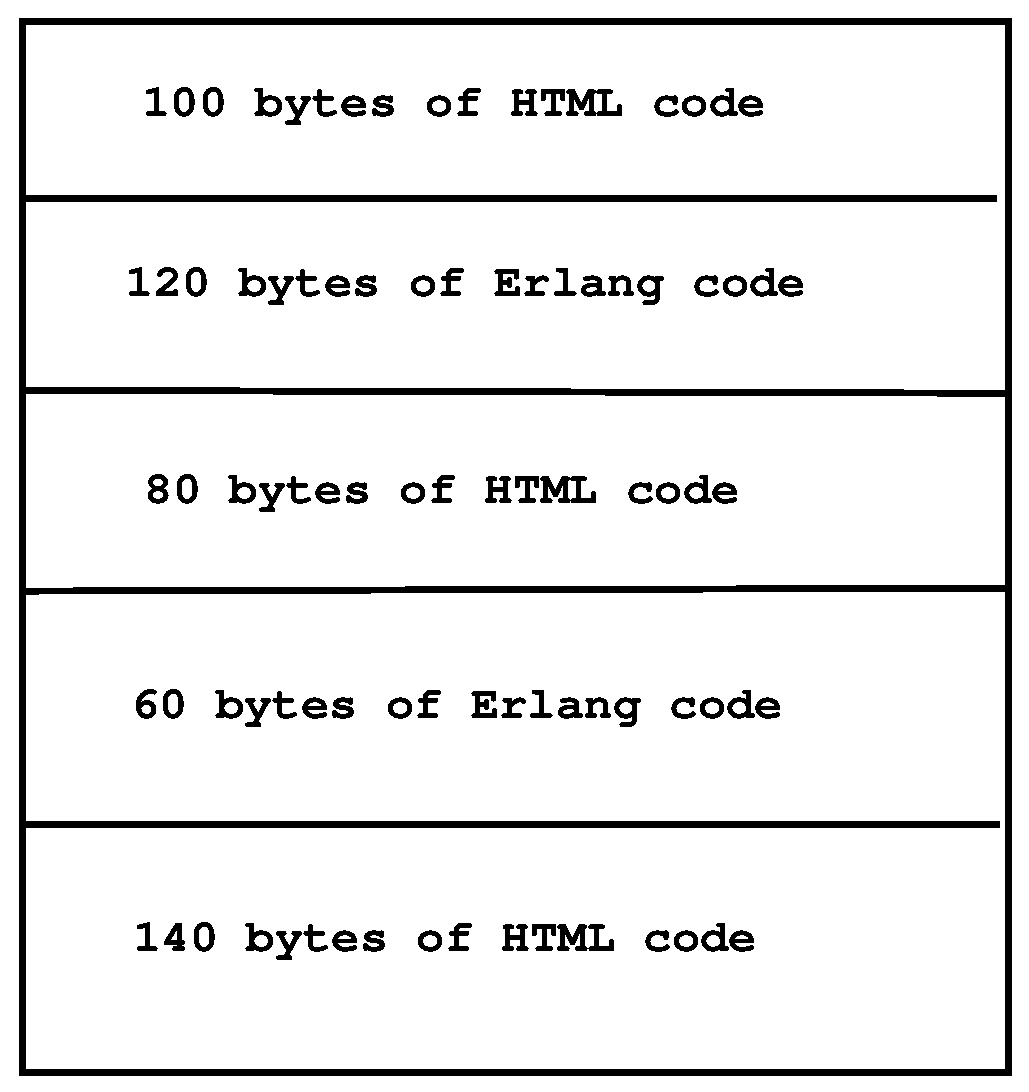
\includegraphics[scale=0.4] {layout}

\end{center}
\end{figure}

The \Yaws\ server will then parse the file and produce a structure
which makes it possible to readily deliver the page without parsing
the next time the same page is requested.

When shipping the page it will
\begin{enumerate}
\item Ship the first 100 bytes from the file
\item Evaluate the first \Erlang\  chunk in the file and ship the output
from the \verb+out/1+ function in that chunk. It will also jump ahead
in the file and skip 120 bytes.
\item Ship 80 bytes of HTML code
\item Again evaluate an \Erlang\  chunk, this time the second and jump
ahead 60 bytes in the file.
\item And finally ship 140 bytes of HTML code to the client
\end{enumerate}

\Yaws\ writes the source output of the compilation into a directory
\verb+/tmp/yaws/$UID+. The beam files are never written to a file.
Sometimes it can be useful to look at the generated source code files,
for example if the \Yaws{}\slash \Erlang\ code contains a compilation
error which is hard to understand.


\section{Evaluating the Yaws Code}

All client requests will execute in their own \Erlang\  process.
For each group of virtual hosts on the same IP:PORT pair
one \Erlang\  process listens for incoming requests.

This process spawns acceptor processes for each incoming request.
Each acceptor process reads and parses all the HTTP headers from the
client. It then looks at the \verb+Host:+ header to figure out which
virtual server to use, i.e. which docroot to use for this particular
request. If the \verb+Host:+ header doesn't match any server from
\textit{yaws.conf} with that IP:PORT pair, the first one from
\textit{yaws.conf} is chosen.

By default \Yaws\  will not ship any data at all to the client
while evaluating a \Yaws\  page. The headers as well as the generated
content are accumulated and not shipped to the client until the
entire page has been processed.


\chapter{SSL}

Secure Socket Layer (SSL) is a protocol used on the Web for delivering
encrypted pages to the WWW client. SSL is widely deployed on the
Internet and virtually all bank transactions as well as all online
shopping today is done with SSL encryption. There are many good
sources on the net that describe SSL in detail, so we will not try to
do that here.  See for example
\url{http://www.tldp.org/HOWTO/SSL-Certificates-HOWTO/}, which
describes how to manage certificates and keys.

In order to run an SSL server we must have a certificate. Either we can
create a so-called self-signed certificate ourselves or buy a certificate
from one of the many CA's (Certificate Authorities) on the net. \Yaws\
uses the SSL application provided by Erlang/OTP and depends on features
supported by it. So, from an Erlang/OTP release to another, some SSL
options may change, others may appear or disappear. Check the
documentation of your Erlang/OTP release for details.

To setup a \Yaws\ server with SSL we could have a \textit{yaws.conf}
file that looks like:

\begin{verbatim}
logdir = /var/log/yaws

<server www.funky.org>
    port = 443
    listen = 192.168.128.32
    docroot = /var/yaws/www.funky.org
    <ssl>
        keyfile = /etc/funky.key
        certfile = /etc/funky.cert
        password = gazonk
    </ssl>
</server>
\end{verbatim}

This is the easiest possible SSL configuration. The configuration
refers to a certificate file and a key file. The certificate file
must contain the name "www.funky.org" as it "Common Name".

The keyfile is the private key file and it is encrypted using
the password "gazonk".


\section{Server Name Indication}

\textbf{The SNI support was introduced in the SSL application in
  Erlang/OTP 18.0}. It is an extension to the TLS protocol (RFC 4366),
which allows the client to include the requested hostname in the first
message of its SSL handshake.

With SNI, you can have many virtual server sharing the same IP address
and port, and each one can have its own unique certificate (and the rest
of the configuration). If SNI is disabled or not supported, all virtual
servers on the same IP/Port must share the same SSL configuration. In
this situation, it is complicated for \Yaws\ to present a valid SSL
certificate to clients. Possible solutions are listed here:
\url{http://wiki.cacert.org/VhostTaskForce}.

By default, SNI is disabled in \Yaws\ to be backward compatible with old
Erlang/OTP releases. But it can be enabled and fine tuned for each SSL
servers. Here is a basic example:


\begin{verbatim}
logdir = /var/log/yaws
sni = enable

<server www.example.com>
    port = 443
    listen = 192.168.128.32
    docroot = /var/yaws/www.example.com
    <ssl>
        keyfile = /etc/ssl/www.example.com.key
        certfile = /etc/ssl/www.example.com.cert
    </ssl>
</server>

<server www.example.org>
    port = 443
    listen = 192.168.128.32
    docroot = /var/yaws/www.example.org
    <ssl>
        keyfile = /etc/ssl/www.example.org.key
        certfile = /etc/ssl/www.example.org.cert
    </ssl>
</server>
\end{verbatim}

Depending on the SNI hostname provided by the client, the first or the
second virtual host will be chosen, and the corresponding SSL
certificate will be presented to the client. In this example, non SNI
clients are still supported. For such clients, the SSL certificate of
the first virtual server will be presented and the HTTP Host header will
be then used to find the correct virtual server. Otherwise, it is
possible to refuse non SNI clients, globally or per server.


\chapter{Applications}

\Yaws\  is well suited for Web applications. In this chapter we will
describe a number of application templates. Code and strategies that
can be used to build Web applications.

There are several ways of starting applications from \Yaws{}.

\begin{itemize}
\item The first and most easy variant is to specify the
  \verb+-r Module+ flag to the \Yaws\ startup script.  This will
  \verb+apply(Module,start,[])+

\item We can also specify \verb+runmods+ in the \textit{yaws.conf}
  file.  It is possible to have several modules specified if want the
  same \Yaws\ server to run several different applications.

\begin{verbatim}

runmod = myapp
runmod = app_number2

\end{verbatim}

\item It is also possible to do it the other way around, let the main
  application start \Yaws{}. We call this embedded mode, which we will
  discuss in chapter \ref{embedded}.

\end{itemize}



\section{Login scenarios}

Many Web applications require the user to login. Once the user has
logged in the server sets a cookie and then the user will be
identified by help of the cookie in subsequent requests.

\subsection{The session server}
The cookie is passed in the headers and is available to the
\Yaws\ programmer in the \verb+Arg+ \verb+#arg+ record. The
\Yaws\ session server can help us to maintain a state for a user while
the user is logged in to the application. The session server has the
following 5 API functions to aid us:

\begin{enumerate}
\item \verb+yaws_api:new_cookie_session(Opaque)+ --- This function
  initiates a new cookie-based session. The \verb+Opaque+ data is
  typically some application-specific structure which makes it
  possible for the application to read a user state, or it can be the
  actual user state itself.

\item \verb+yaws_api:cookieval_to_opaque(Cookie)+ --- This function
  maps a cookie to a session.

\item \verb+yaws_api:replace_cookie_session(Cookie, NewOpaque)+ ---
  Replace the opaque user state in the session server with
  \verb+NewOpaque+.

\item \verb+yaws_api:delete_cookie_session(Cookie)+ --- This function
  should typically be called when the user logs out or when our web
  application decides to automatically logout the user.

\end{enumerate}

All cookie-based applications are different but they have some things
in common. In the following examples we assume the existence of a
function \verb+myapp:auth(UserName, Passwd)+ and it returns \verb+ok+
or \verb+{error, Reason}+.

Let's assume the following record:

\begin{verbatim}

-record(session, {user,
                  passwd,
                  udata = []}).

\end{verbatim}

The following function is a good template function to check the
cookie.

\begin{verbatim}

get_cookie_val(CookieName, Arg) ->
    H = Arg#arg.headers,
    yaws_api:find_cookie_val(CookieName, H#headers.cookie).



check_cookie(A, CookieName) ->
    case get_cookie_val(CookieName, A) of
        []  ->
            {error, "not logged in"};
        Cookie ->
            yaws_api:cookieval_to_opaque(Cookie)
    end.

\end{verbatim}

We need to check all requests and make sure the session\_server has
our cookie registered as an active session. Also, if a request comes
in without a working cookie we want to present a login page instead of
the page the user requested. Another quirky issue is that the pages
necessary for display of the login page must be shipped without
checking the cookie. The next sections explain how these needs can be
met.

\subsection{Arg rewrite}

In this section we describe a feature whereby the user is allowed to
rewrite the \verb+Arg+ at an early stage in the \Yaws\ server.  We do
that by specifying an \verb+arg_rewrite_mod+ in the \textit{yaws.conf}
file.

\begin{verbatim}
arg_rewrite_mod = myapp
\end{verbatim}


Then in the \verb+myapp+ module we have:

\begin{verbatim}
arg_rewrite(Arg) ->
    OurCookieName = "myapp_sid"
    case check_cookie(A, OurCookieName) of
        {error, _} ->
            do_rewrite(Arg);
        {ok, _Session} ->
            %return Arg untouched
            Arg
    end.

%% these pages must be shippable without a good cookie
login_pages() ->
    ["/banner.gif", "/login.yaws", "/post_login.yaws"].

do_rewrite(Arg) ->
    Req = Arg#arg.req,
    {abs_path, Path} = Req#http_request.path,
    case lists:member(Path, login_pages()) of
        true ->
            Arg;
        false ->
            Arg#arg{req = Req#http_request{path = {abs_path, "/login.yaws"}},
                    state = Path}
    end.

\end{verbatim}

Our arg rewrite function lets all \verb+Arg+s go through untouched
that either have a good cookie or belong to a set of predefined pages
that are acceptable to get without being logged in.  If we decide that
the user must log in, we change the path of the request, thereby
making the \Yaws\ server ship a login page instead of the page the
user requested. We also set the original path in the \verb+Arg+ state
argument so that the login page can redirect the user to the original
page once the login procedure is finished.

Within an arg rewrite function, examining and modifying HTTP headers can be
achieved using the following functions from the \verb+yaws_api+ module:

\begin{itemize}
\item \verb+set_header/2+, \verb+set_header/3+
\item \verb+get_header/2+, \verb+get_header/3+
\item \verb+merge_header/2+, \verb+merge_header/3+
\item \verb+delete_header/2+
\end{itemize}

All functions operate on instances of the \verb+#headers{}+ record type
defined in the \verb+yaws_api.hrl+ include file.

Should an arg rewrite function need to return a response for a particular
request, it can do so by returning an \verb+#arg+ record instance with its
\verb+state+ field set to an instance of a \verb+#rewrite_response+
record. For example, below is an arg rewrite function that allows only
\verb+GET+ and \verb+POST+ requests, returning a 405 \emph{Method Not
  Allowed} for requests with any other HTTP method:

\begin{verbatim}
arg_rewrite(Arg) ->
    Allowed = ['GET', 'POST'],
    Req = yaws_api:arg_req(Arg),
    Method = yaws_api:http_request_method(Req),
    case lists:member(Method, Allowed) of
        true ->
            Arg;
        false ->
            AllowedStrs = string:join([atom_to_list(M) || M <- Allowed], ","),
            Arg#arg{state=
                        #rewrite_response{
                           status=405,
                           headers=[{header, {"Allow", AllowedStrs}},
                                    {header, {connection, "close"}}]}}
    end.
\end{verbatim}

\subsection{Authenticating}

Now we're approaching the \verb+login.yaws+ page, the page that
displays the login prompt to the user. The login page consists of two
parts: one part that displays the login data as a form, and one form
processing page that reads the data the user entered in the login
fields and performs the actual authentication.

The login page performs a tiny well-known Web trick where it passes
the original URL request in a hidden field in the login page and
thereby passing that information to the form processing page.

The page \verb+login.yaws+:

\begin{verbatim}
<erl>

out(A) ->
    {ehtml,
     {html,[],
      [{h2, [], "Login page"},
       {hr},
       {form, [{action,"/login_post.yaws"},
               {method,post}],

        [{p,[], "Username"}, {input, [{type,text},{name,uname}]},
         {p,[],"Password"},  {input, [{type,password},{name,passwd}]},
         {input, [{type,submit},{value,"Login"}]},
         {input, [{type,hidden},{name,url},
                  {value, A#arg.state}]}]}]}}.

</erl>
\end{verbatim}



The form processing page which gets the \verb+POST+ data from the code
above:

\begin{verbatim}


<erl>

-include("myapp.hrl").
%% we have the session record there
%% we must set the include_path in the yaws.conf file
%% in order for the compiler to find that file

kv(K,L) ->
    {value, {K, V}} = lists:keysearch(K,1,L),
    V.

out(A) ->
    L = yaws_api:parse_post(A),
    User = kv(user, L),
    Pwd =  kv(passwd, L),
    case myapp:auth(User, Pwd) of
        ok ->
            S = #session{user = User,
                         passwd = Pwd,
                         udata = []},
            %% Now register the session to the session server
            Cookie = yaws_api:new_cookie_session(S),
            [{redirect_local, kv(url, L)},
              yaws_api:set_cookie("myapp_sid",Cookie,[])]
        Err ->
            {ehtml,
             {html, [],
              {p, [], f("Bad login: ~p",[Err])}}}
    end.

</erl>



\end{verbatim}

The function returns a list of two new (not previously discussed)
return values: instead of returning HTML output as in
\verb+{html, Str}+ or \verb+{ehtml,Term}+ we return a list of two new
values. (There are many different possible return values from the
\verb+out/1+ function and they will all be described later.) The two
new values are:

\begin{enumerate}

\item The tuple \verb+{redirect_local, Path}+ makes the \Yaws\ web
  server return a 302 redirect to the specified \verb+Path+.
  Optionally a different status code can be supplied which will be
  used in place of 302, e.g.  \verb+{redirect_local, Path, 307}+.

\item \verb+yaws_api:set_cookie("myapp_sid",Cookie,[])+ generates a
  \verb+Set-Cookie+ header.
\end{enumerate}

Now if we put all this together we have a full-blown cookie-based
login system. The last thing we did in the form processing code was
to register the session with the session server thereby letting any
future requests go straight through the \verb+Arg+ rewriter.

This way both \Yaws\  pages as well as all or some static content
is protected by the cookie login code.

\subsection{Database driven applications}

We can use code similar to the code in the previous section to associate
a user session to entries in a database. Mnesia fits perfectly
together with \Yaws\  and keeping user persistent state in Mnesia is
both easy and convenient.

Once the user has logged in we can typically use the user name as key
into the database. We can mix \verb+ram_tables+ and \verb+disc_tables+
to our liking. The Mnesia database must be initialized via
\verb+create_table/2+ before it can be used. This is typically done
while installing the web application on a machine.

Another option is to let the application check that Mnesia
is initialized whenever the application starts.

If we don't want or need to use Mnesia, it's of course possible
to use a simple \verb+dets+ file or a text file as well.

\section{Appmods}
\label{appmods}

Appmods is mechanism to invoke different applications based upon the
URL. A URL---as presented to the web server in a request---has a path
part and a query part.

It is possible to install several appmods in the \textit{yaws.conf}
file as shown below:

\begin{verbatim}

appmods = foo myapp

\end{verbatim}

Now, if the user requests a URL where any component in the
directory path is an appmod, the parsing of the URL will terminate
there and instead of reading the actual file from the disk, \Yaws\  will
invoke the appmod with the remainder of the path inserted into
\verb+Arg#arg.appmoddata+.

Say the user requests the URL
\url{http://www.funky.org/myapp/xx/bar.html}.  \Yaws\ will not ship
the file \verb+bar.html+ to the client, instead it will invoke
\verb+myapp:out(Arg)+ with \verb+Arg#arg.appmoddata+ set to the string
\verb+xx/bar.html+. Any optional query data---that is, data that
follows the first '?' character in the URL---is removed from the path
and passed as \verb+Arg#arg.querydata+.

Appmods can be used to run applications on a server. All requests
to the server that has an appmod in the URL will be handled by that
application. If the application decides that it want to
ship a page from the disk to the client, it can return the
tuple \verb+{page, Path}+. This return value will make \Yaws\  read
the page from the disk, possibly add the page to its cache of
commonly accessed pages and ship it back to the client.

The \verb+{page, Path}+ return value is equivalent to a
redirect, but it removes an extra round trip, and is thus faster.

Appmods can also be used to fake entire directory hierarchies
that don't exist on disk.


\section{The opaque data}

Sometimes an application needs application-specific data such as the
location of its data files. There exists a mechanism to pass
application-specific configuration data from the \Yaws\ server to the
application.

When configuring a server we have an opaque field in the configuration
file that can be used for this purpose.  Say we have the following
fields in the config file:

\begin{verbatim}

<server foo>
    listen = 192.168.128.44
    <opaque>
        foo = bar
        somefile = /var/myapp/db
        myname = hyber
    </opaque>
</server>
\end{verbatim}

This will create a normal server that listens to the specified IP address.
An application has access to the opaque data that was specified
in that particular server through \verb+Arg#arg.opaque+.

If we have the opaque data specified above, the \verb+Arg+ opaque
field will have the value:

\begin{verbatim}

[{foo, "bar"},
 {somefile, "/var/myapp/db"},
 {myname, "hyber"}
]

\end{verbatim}


\section{Customizations}

When actually deploying an application at a live site, some of the
standard \Yaws\ behaviors are not acceptable. Many sites want to
customize the web server behavior when a client requests a page that
doesn't exist on the web server. The standard \Yaws\ behavior is to
reply with status code 404 and a message explaining that the page
doesn't exist.

Similarly, when \Yaws\  code crashes, the reason for the crash is
displayed in the Web browser. This is very convenient while
developing a site but not acceptable in production.


\subsection{404 File not found}

We can install a special handler for 404 messages. We do that by
specifying a \verb+errormod_404+ in the \textit{yaws.conf} file.

If we have:

\begin{verbatim}
<server foo>
  ..
  ..
  ..
  errormod_404 = myapp

</server>

\end{verbatim}

When \Yaws\ gets a request for a file that doesn't exist, it invokes
the \verb+errormod_404+ module to generate both the status code as
well as the content of the message.

If \verb+Module+ is specified as the \verb+errormod_404+ module,
\Yaws\ will invoke \verb+Module:out404(Arg, GC, SC)+, passing the
arguments as described below:

\begin{itemize}
\item \verb+Arg+ is an \verb+#arg{}+ record

\item \verb+GC+ is a \verb+#gconf{}+ record (defined in \verb+yaws.hrl+)

\item \verb+SC+ is a \verb+#sconf{}+ record (defined in
  \verb+yaws.hrl+)
\end{itemize}

The function can and must do the same things that a normal
\verb+out/1+ function does.


\subsection{Crash messages}

We use a similar technique for generating the crash messages: we
install a module in the \textit{yaws.conf} file and let that module
generate the crash message.  We have:

\begin{verbatim}
errormod_crash = Module
\end{verbatim}

The default is to display the entire formatted crash message in the
browser.  This is good for debugging but not good for production.

If \verb+Module+ is specified as the \verb+errormod_crash+ module, the
function \verb+Module:crashmsg(Arg, SC, Str)+ will be called.  The
\verb+Str+ argument is the real crash message formatted as a string.

\section{Stream content}

If the \verb+out/1+ function returns the tuple
\verb+{content, MimeType, Content}+ \Yaws\ will ship that data to the
Client. This way we can deliver dynamically generated content to the
client which is of a different MIME type than "text/html".

If the generated response is very large and it not possible or
practical to generate the whole thing, we can return the value:

\begin{verbatim}
{streamcontent, MimeType, FirstChunk}
\end{verbatim}

\noindent which delivers data back to the client using HTTP chunked
transfer (see RFC 2616 section 3.6.1) and then from a different
\Erlang\ process deliver the remaining chunks by using the functions
described below:

\begin{enumerate}
\item \verb+yaws_api:stream_chunk_deliver(YawsPid, Data)+ where the
  \verb+YawsPid+ is the process id of the \Yaws\ worker process. That
  pid is available in \verb+Arg#arg.pid+.

\item \verb+stream_chunk_end(YawsPid)+ which must be called to
  indicate the end of the stream.
\end{enumerate}

A streaming alternative is also available for applications that need a
more direct way to deliver data to clients, such as those dealing with
data too large to buffer in memory but not wishing to use chunked
transfer, or applications that use long-polling (Comet) techniques
that require them to hold client connections open for extended
periods. For these situations we can return the value:

\begin{verbatim}
{streamcontent_from_pid, MimeType, Pid}
\end{verbatim}

\noindent to tell \Yaws\ we wish to deliver data of MIME type
\verb+MimeType+ to the client from process \verb+Pid+. In this case,
\Yaws\ will prepare the socket for delivery from \verb+Pid+ and then
send one of the following messages to \verb+Pid+:
\begin{itemize}
\item \verb+{ok, YawsPid}+ tells \verb+Pid+ that it is now OK to
  proceed with sending data back to the client using the socket. The
  socket is accessible as \verb+Arg#arg.clisock+.

\item \verb+{discard, YawsPid}+ informs \verb+Pid+ that it should not
  attempt to use the socket, typically because the requested HTTP
  method requires no response body.
\end{itemize}

We call one of the following functions to send data:
\begin{itemize}
\item \verb+yaws_api:stream_process_deliver(Socket, IoList)+ sends data
  \verb+IoList+ using socket \verb+Socket+ without chunking the data. To
  ensure chunking is not in effect, return

\begin{verbatim}
{header, {transfer_encoding, erase}}
\end{verbatim}

  in a list with the \verb+streamcontent_from_pid+ directive (which must
  always be last in such a list).

\item \verb+yaws_api:stream_process_deliver_chunk(Socket, IoList)+
  sends data \verb+IoList+ using socket \verb+Socket+ but converts
  the data into chunked transfer form before sending it.
\end{itemize}

Pids using chunked transfer must indicate the end of their transfer by
calling the following function:
\begin{itemize}
\item \verb+yaws_api:stream_process_deliver_final_chunk(Socket, IoList)+
\end{itemize}

which delivers a special HTTP chunk to mark the end of the data
transfer to the client.

Finally, \verb+Pid+ must always call
\verb+yaws_api:stream_process_end(Socket, YawsPid)+ when it finishes
sending data or when it receives the \verb+{discard, YawsPid}+ message
from \Yaws\ --- this is required to inform \Yaws\ that \verb+Pid+ has
finished with the socket and will not use it directly anymore. If the
application has to close the socket while it's in control of it,
though, it must pass the atom \verb+closed+ as the first argument to
\verb+yaws_api:stream_process_end+ in place of the socket to inform
\Yaws\ that the socket has been closed and it should no longer attempt
to use it.

App\-li\-ca\-tions that use the \verb+streamcontent_from_pid+
directive that also want to a\-void chunked transfer encoding for
their streams should be sure to include a set\-ting for the
\verb+Content-Length+ header in their \verb+out/1+ return
value. \Yaws\ au\-to\-mat\-i\-cal\-ly sets the
\verb+Transfer-Encoding+ head\-er to \verb+chunked+ if it does not
detect a \verb+Content-Length+ header.

\section{All out/1 return values}

\begin{itemize}


\item \verb+{html, DeepList}+ This assumes that \verb+DeepList+ is
  formatted HTML code.  The code will be inserted in the page.

\item \verb+{ehtml, Term}+ This will transform the \Erlang\ term
  \verb+Term+ into a stream of HTML content.

\item \verb+{exhtml, Term}+ This will transform the \Erlang\ term
  \verb+Term+ into a stream of strict XHTML code.

\item \verb+{content, MimeType, Content}+ This function will make the
  web server generate different content than HTML. This return value
  is only allowed in a \Yaws\ file which has only one
  \verb+<erl> </erl>+ part and no html parts at all.

\item \verb+{streamcontent, MimeType, FirstChunk}+ This return value
  plays the same role as the \verb+content+ return value above.
  However it makes it possible to stream data to the client using HTTP
  chunked transfer if the \Yaws\ code doesn't have access to all the
  data in one go. (Typically if a file is very large or if data
  arrives from back end servers on the network.)

\item
  \verb+{streamcontent_with_timeout, MimeType, FirstChunk, Timeout}+
  Similar to the above, but with an explicit timeout. The default
  timeout is 30 secs, i.e. if the application fails to deliver data to
  the \Yaws\ process, the streaming will stop. This is often not the
  desired behaviour in Comet/Ajax applications. It's possible to
  provide 'infinity' as the timeout.

\item \verb+{streamcontent_from_pid, MimeType, Pid}+ This return value
  is similar to the \verb+streamcontent+ return value above.  However
  it makes it possible to stream data to the client directly from an
  application process to the socket. This approach can be useful for
  applications that employ long-polling (Comet) techniques, for
  example, and for applications wanting to avoid buffering data or
  avoid HTTP chunked mode transfer for streamed data.

\item \verb+{streamcontent_with_size, Sz, MimeType, Pid}+ This is
  similar to the \verb+streamcontent+ return value above. However it
  makes it possible to stream data to the client by setting the
  content length of the response. As the opposite of other ways to
  stream data, in this case, the response is not chunked encoded.


\item \verb+{header, H}+ Accumulates a HTTP header. The trailing CRNL which is
  supposed to end all HTTP headers must NOT be added. It is added by the server.
  The following list of headers are given special treatment.

  \begin{itemize}
    \item \verb+{connection, What}+ - This sets the Connection: header. If
      \textit{What} is the special value \textit{\"close\"}, the connection will
      be closed once the yaws page is delivered to the client.
    \item \verb+{server, What}+ - Sets the \textit{Server:} header. By setting
      this header, the server's signature will be dynamically overloaded.
    \item \verb+{location, What}+ - Sets the \textit{Location:} header. This
      header is typically combined with the \textit{\{status, 302\}} return
      value.
    \item \verb+{cache_control, What}+ - Sets the \textit{Cache-Control:}
      header.
    \item \verb+{expires, What}+ - Sets the \textit{Expires:} header.
    \item \verb+{date, What}+ - Sets the \textit{Date:} header.
    \item \verb+{allow, What}+ - Sets the \textit{Allow:} header.
    \item \verb+{last_modified, What}+ - Sets the \textit{Last-Modified:}
      header.
    \item \verb+{etag, What}+ - Sets the \textit{Etag:} header.
    \item \verb+{set_cookie, What}+ - Prepends a \textit{Set-Cookie:} header to
      the list of previously set \textit{Set-Cookie} headers.
    \item \verb+{content_range, What}+ - Sets the \textit{Content-Range:}
      header.
    \item \verb+{content_type, What}+ - Sets the \textit{Content-Type:} header.
    \item \verb+{content_encoding, What}+ - Sets the \textit{Content-Encoding:}
      header. If this header is defined, no deflate is performed by \Yaws\. So
      you can compress data by yourself.
    \item \verb+{content_length, What}+ - Normally \Yaws\ will ship Yaws pages
      using \textit{Transfer-Encoding: chunked}. This is because we generally
      can't know how long a yaws page will be. If we for some reason want to
      force a \textit{Content-Length:} header (and we actually do know the
      length of the content, we can force yaws to not ship the page chunked.
    \item \verb+{transfer_encoding, What}+ - Sets the
      \textit{Transfer-Encoding:} header.
    \item \verb+{www_authenticate, What}+ - Sets the \textit{WWW-Authenticate:}
      header.
    \item \verb+{vary, What}+ - Sets the \textit{Vary:} header.
  \end{itemize}

  All other headers must be added using the normal HTTP syntax. Example:
\begin{verbatim}
{header, {"My-X-Header", "gadong"}} or {header, "My-X-Header: gadong"}
\end{verbatim}

\item \verb+{header, {H, erase}}+ A specific case of the previous
  directive; use this to remove a specific header from a response. For
  example, streaming applications and applications using server-sent events
  (see \url{http://www.w3.org/TR/eventsource/ }) should use
  \verb+{header, {transfer_encoding, erase}}+ to turn off chunked encoding
  for their responses.

\item \verb+{allheaders, HeaderList}+ Will clear all previously
  accumulated headers and replace them.

\item \verb+{status, Code}+ Sets the response HTTP status code to
  \verb+Code+.

\item \verb+break+ Will stop processing of any consecutive chunks of
  erl or HTML code in the \Yaws\ file.

\item \verb+ok+ Do nothing.

\item \verb+flush+ Flush remaining data sent by the client.

\item \verb+{redirect, Url}+ Erase all previous headers and accumulate
  a single HTTP \verb+Location+ header. Set the status code to 302.

\item \verb+{redirect, Url, Status}+ Same as redirect above with the
  additional option of supplying the status code. The default for a
  redirect is 302 but 301, 303 and 307 are also valid redirect status
  codes.

\item \verb+{redirect_local, Path}+ Does a redirect to the same
  \url{Scheme://Host:Port/Path} in which we are currently
  executing. \verb+Path+ can be either be the path directly
  (equivalent to \verb+abs_path+), or one of \verb+{{abs_path, Path}+
  or \verb+{{rel_path, RelativePath}}+

\item \verb+{redirect_local, Path, Status}+ Same as
  \verb+redirect_local+ above with the additional option of supplying
  the status code. The default for a redirect is 302 but 301, 303 and
  307 are also valid redirect status codes.

\item \verb+{get_more, Cont, State}+ When we are receiving large
  \verb+POST+s we can return this value and be invoked again when more
  data arrives.

\item \verb+{page, Page}+ Make \Yaws\ returns a different local page than the
  one being requested. \verb+Page+ is a Request-URI, so it must be url-encoded
  and can contain a query-string.

\item \verb+{page, {Options, Page}}+ Like the above, but supplying an
  additional deep list of options.  Supported options types are:

  \begin{itemize}
    \item \verb+{status, C}+ - Set the HTTP response status code \verb+C+ for
      page \verb+Page+.
    \item \verb+{header, H}+ - Accumulate the HTTP header \verb+H+ for page
      \verb+Page+.
    \item \verb+{disable_cache, Bool}+ - if set to \verb+true+, disable the
      cache of \verb+Page+ for this call.
  \end{itemize}

\item \verb+{websocket, CallbackModule, Options}+ Tell \Yaws\  to use
  \verb+CallbackModule+ as a WebSockets Protocol handler for traffic
  on the client socket. See chapter \ref{websockets} for more details.

\item \verb+[ListOfValues]+ It is possible to return a list of the above defined
  return values. Any occurrence of the atoms \verb+streamcontent+,
  \verb+streamcontent_with_timeout+,
  \verb+streamcontent_with_size+,\\
  \verb+streamcontent_from_pid+, \verb+get_more+, \verb+page+ or \verb+break+ in
  this list is legal only if it is the last position of the list. If not,
  remaining values in the list are ignored.

\end{itemize}



\chapter{Debugging and Development}

\Yaws\ has excellent debugging capabilities. First and foremost we
have the ability to run the web server in interactive mode by means of
the command line switch \verb+-i+, which gives us a regular
\Erlang\ command line prompt we can use to compile helper code or
reload helper code. Furthermore all error messages are displayed
there.  If a \verb+.yaws+ page producees any regular \Erlang\ I\slash
O, that output will be displayed at the \Erlang\ prompt, assuming we
are running in interactive mode.

If we give the command line switch \verb+-d+ we get some additional
error messages. Also \Yaws\ does some additional checking of user
supplied data such as headers.

\section{Logs}
\Yaws\ produces various logs. All log files are written into the
\Yaws\ logdir directory. This directory is specified in the config
file.

We have the following log files:

\begin{itemize}
\item The access log. Access logging is turned on or off per server in
  the \textit{yaws.conf} file. If access\_log is turned on for a
  server, \Yaws\ will produce a log in Common Access Log Format called
  \textit{HostName:PortNumber.access}

\item The auth log. Auth logging is turned on or off per server in the
  \textit{yaws.conf} file. If auth\_log is turned on for a server,
  \Yaws\ will produce a log called \textit{HostName:PortNumber.auth}
  which contains all HTTP auth-related messages.

\item \textit{report.log} This file contains all error and crash
  messages for all virtual servers in the same file.

\item Trace files. The two command line flags \verb+-t+ and \verb+-T+ tells
\Yaws\ to trace all traffic or just all HTTP messages and write them to files.
\end{itemize}


\chapter{External scripts via CGI}

\Yaws\  can also interface to external programs generating dynamic
content via the Common Gateway Interface (CGI).  This has to be
explicitly enabled for a virtual host by listing \verb+cgi+ in the
\verb+allowed_scripts+ line in the configuration file.  Any request
for a page ending in \verb+.cgi+ (or \verb+.CGI+) will then result in
trying to execute the corresponding file.

If you have a PHP executable compiled for using CGI in the \verb+PATH+
of the \Yaws\  server, you can enable PHP support by adding \verb+php+ to
\verb+allowed_scripts+.  Requests for pages ending in \verb+.php+ will
then result in \Yaws\  executing \verb+php+ (configurable via
\verb+php_handler+) and passing the name of the corresponding file to
it via the appropriate environment variable.

These ways of calling CGI scripts are also available to \verb+.yaws+
scripts and appmods via the functions \verb+yaws_api:call_cgi/2+ and
\verb+yaws_api:call_cgi/3+.  This makes it possible to write wrappers
for CGI programs, irrespective of the value of \verb+allowed_scripts+.

The author of this \Yaws\  feature uses it for self-written CGI programs
as well as for using a standard CGI package.  You should not be
surprised however, should some scripts not work as expected due to an
incomplete or incorrect implementation of certain CGI meta-variables.
The author of this feature is interested in hearing about your
experiences with it.  He can be contacted at \verb+carsten@codimi.de+.

\chapter{FastCGI}

\Yaws\  supports the responder role and the authorizer role of the
FastCGI protocol. See \verb+www.fastcgi.com+ for details on the
FastCGI protocol.

The benefits of using FastCGI include:
\begin{enumerate}
\item Unlike CGI, it is not necessary to spawn a new process for
every request; the application server can handle multiple requests
in a single process.
\item The fact that the application server can run on a different
computer benefits scalability and security.
\item The application server can be written in any language for
which a FastCGI library is available. Existing applications
which have been written for other web servers can be used with
\Yaws{}.
\item FastCGI can also be used to implement external authentication
servers (in addition to generating dynamic content).
\end{enumerate}

Support for FastCGI was added to \Yaws\  by Bruno Rijsman
(\verb+brunorijsman@hotmail.com+).

\section{The FastCGI Responder Role}

The FastCGI responder role allows \Yaws\  to communicate with an
application server running on a different (or on the same) computer
to generate dynamic content.

The FastCGI protocol (which runs over TCP) is used to send the request
information from \Yaws\  to the application server and to send the
response information (e.g. the generated dynamic content) from
the application server back to \Yaws{}.

FastCGI responders can be invoked in two ways:

\begin{enumerate}

\item
By including \verb+fcgi+ in the \verb+allowed_scripts+ line
in the configuration file (note that the default value for
\verb+allowed_scripts+ includes \verb+fcgi+).

In this case a request for any resource with the \verb+.fcgi+
extension will result in a FastCGI call to the application server to
dynamically generate the content.

Note: the \Yaws\  server will only call the application server if a file
corresponding to the resource name (i.e. a file with the \verb+.fcgi+
extension) exists locally on the \Yaws\  server. The contents of that
file are not relevant.

\item
By creating an appmod which calls \verb+yaws_api:call_fcgi_responder+.
See the \verb+yaws_api(5)+ man page for details.

\end{enumerate}

\section{The FastCGI Authorizer Role}

The FastCGI authorizer role allows \Yaws\  to communicate with an
authentication server to authenticate requests.

The FastCGI protocol is used to send the request information from
\Yaws\ to the authentication server and the authentication response
back from the authentication server to \Yaws{}.

If access is allowed, \Yaws\ proceeds to process the request normally.

If access is denied, the authentication server provides the
response which is sent back to the client. This is typically
a ``not authorized'' response or a redirect to a login page.

FastCGI authorizers are invoked by creating an appmod which
calls \verb+yaws_api:call_fcgi_authorizer+.
See the \verb+yaws_api(5)+ man page for details.

\section{The FastCGI Filter Role}

FastCGI defines a third role, the filter role, which
\Yaws\  does not currently support.


\section{FastCGI Configuration}

The following commands in the \textit{yaws.conf} file control the
operation of FastCGI.

If you use FastCGI, you \emph{must} include the \verb+fcgi_app_server+
setting in the configuration file to specify the host name (or IP address)
and TCP port of the FastCGI application server.

You may include the \verb+fcgi_trace_protocol+ setting to enable or disable
tracing of FastCGI protocol messages. This is useful for debugging.

You may include the \verb+fcgi_log_app_error+ setting to enable or disable
logging application errors (any output to stderr and non-zero exit codes).

You may include the \verb+extra_cgi_vars+ command to pass additional
environment variables to the application.


\chapter{Security}

\Yaws\  is of course susceptible to intrusions. \Yaws\  has the
ability to run under a different user than root, even if we need
to listen to privileged port numbers. Running as root is generally a
bad idea.

Intrusions can happen basically at all places in \Yaws\ code where the
\Yaws\ code calls either the BIF \verb+open_port+ or when \Yaws\ code
calls \verb+os:cmd/1+. Both \verb+open_port+ and \verb+os:cmd/1+
invoke the \verb+/bin/sh+ interpreter to execute its commands. If the
commands are nastily crafted bad things can easily happen.

All data that is passed to these two function must be carefully
checked.

Since \Yaws\  is written in \Erlang\  a large class of cracks are
eliminated since it is not possible to perform any buffer overrun
cracks on a \Yaws\  server. This is very good.


Another possible point of entry to the system is by providing a URL
which takes the client out from the docroot. This should not be
possible -- and the impossibility relies on the correctness of the URL
parsing code in \Yaws{}.

\section{WWW-Authenticate}
\Yaws\  has support for WWW-Authentication.   WWW-Authenticate is a
standard HTTP scheme for the basic protection of files with a username
and password.  When a client browser wants a protected file, it must send a
\verb+Authenticate: username:password+ header in the request.  Note that
this is plain text.   If there is no such header or the username and
password is invalid the server will respond with status code 401 and
the realm.  Browsers will then tell the user that a username and
password is needed for ``realm'',  and will resend the request after
the user enters the information.

WWW-Authentication is configured in the \textit{yaws.conf} file, in as
many \textit{<auth>} directives as you desire:

\begin{verbatim}
<server foo>
  docroot = /var/yaws/www/

..
..

  <auth>
    realm = secretpage
    dir   = /protected
    dir   = /anotherdir
    user  = klacke:gazonk
    user  = jonny:xyz
    user  = ronny:12r8uyp09jksfdge4
  </auth>
</server>
\end{verbatim}


\Yaws\  will require one of the given username:password pairs for all
files in the \textit{/protected} and \textit{/anotherdir} directories.
Note that these directories are specified as a server path,  that is,
the filesystem path that is actually protected here is
\textit{/var/yaws/www/protected} .


\chapter {Embedded mode}
\label{embedded}

\Yaws\  is a normal OTP application. It is possible to integrate \Yaws\
into another larger application. The \Yaws\  source tree must be
integrated into the larger application's build environment. \Yaws\  is
then simply started by \verb+application:start()+ from the larger
application's boot script, or the \Yaws\  components needed for the
larger application can be started individually under the application's
supervisor(s).

By default \Yaws\ reads its configuration data from a config file, the
default is \textit{/usr/local/etc/yaws/yaws.conf} . If \Yaws\ is integrated
into a larger application, however, that application typically has its
configuration data kept at some other centralized place. Sometimes we
may not even have a file system to read the configuration from if we
run a small embedded system.

\Yaws\  reads its application environment. If the environment key
\verb+embedded+ is set to \verb+true+, \Yaws\  starts in embedded mode.
Once started it must be fed a configuration, and that can be done
after \Yaws\  has started by means of the function
\verb+yaws_api:setconf/2+.

It is possible to call \verb+setconf/2+ several times to force \Yaws\  to
reread the configuration.

\section{Creating Global and Server Configurations}

The \verb+yaws_api:setconf/2+ function mentioned in the previous
section takes two arguments:

\begin{itemize}

\item a \verb+#gconf+ record instance, specifying global
  \Yaws\ configuration

\item a list of lists of \verb+#sconf+ record instances, each
  specifying configuration for a particular server instance

\end{itemize}

These record types are specified in \verb+yaws.hrl+, which is not
normally intended for inclusion by applications. Instead,
\Yaws\  provides the \verb+yaws_api:embedded_start_conf/1,2,3,4+
functions that allow embedded mode applications to specify
configuration data using property lists (lists of
\verb+{key, value}+ pairs).

The \verb+yaws_api:embedded_start_conf+ functions all return a tuple
containing the following four items:

\begin{itemize}

\item the atom \verb+ok+.

\item a list of lists of \verb+#sconf+ record instances. This variable
  is intended to be passed directly to\\* \verb+yaws_api:setconf/2+ as
  its second argument.

\item a \verb+#gconf+ record instance. This variable is intended to
  be passed directly to \verb+yaws_api:setconf/2+ as its first
  argument.

\item a list of supervisor child specification for the
  \Yaws\  components the embedded mode application's configuration
  specified should be started. This allows embedded mode applications
  to start \Yaws\  under its own supervisors.

\end{itemize}

Note that \verb+yaws_api:embedded_start_conf+ does not actually start
any servers, but rather it only returns the configuration information
and child specifications needed for the embedded mode application to
start and configure \Yaws\  itself.

If you have difficulty figuring out how to set up your \verb+#gconf+
or \verb+#sconf+ records for embedded mode, you should first consider
getting something running in non-embedded mode using a
\verb+yaws.conf+ file. Once you're satisfied with the setup and
\Yaws\  is running, execute the following command:

\begin{verbatim}
yaws --running-config
\end{verbatim}

This command will show the \Yaws\ configuration from your
\verb+yaws.conf+ file in terms of \verb+#gconf+ and \verb+#sconf+
records, thus showing you how to set up those records for embedded
mode.

\section{Starting Yaws in Embedded Mode}

An embedded mode application can start \Yaws\  in one of two ways:

\begin{itemize}

\item It can call \verb+yaws_api:embedded_start_conf+ to obtain
  configuration and \Yaws\  startup information as described in the
  previous section, start \Yaws\  under its own supervisors, and then
  pass the global and server configuration settings to
  \verb+yaws_api:setconf/2+.

\item It can call \verb+yaws:start_embedded/1,2,3,4+, each of which
  takes exactly the same arguments as the corresponding
  \verb+yaws_api:embedded_start_conf/1,2,3,4+ function. Instead of just
  returning start and configuration information, however,
  \verb+yaws:start_embedded+ also starts and configures \Yaws{}, which
  can be more convenient but does not allow the embedded mode
  application any supervision control over \Yaws{}.

\end{itemize}

Both of these functions take care of setting the environment key
\verb+embedded+ to \verb+true+. Neither approach requires any special
settings in the embedded mode application's \textit{.app} file nor any
special command-line switches to the \Erlang\  runtime.

For an example of how to use \verb+yaws_api:embedded_start_conf+ along
with \verb+yaws_api:setconf+, please see the files
\verb+www/ybed_sup.erl+ and \verb+www/ybed.erl+ in the
\Yaws\  distribution.

\chapter{The config file - yaws.conf}

In this section we provide a complete listing of all possible
configuration file options.  The configuration contains two distinct
parts: a global part which affects all the virtual hosts and a server
part where options for each virtual host is supplied.

\section{Global Part}

\begin{itemize}


\item       \verb+logdir = Directory+ ---
              All \Yaws\  logs will be  written  to  files  in  this
              directory.  There  are  several different log files
              written by \Yaws{}.

              \begin{itemize}
              \item \verb+report.log+ --- this is a text file that contains  all
              error logger printouts from \Yaws{}.
              \item \verb+<Host>.access+ --- for each virtual host served
                by \Yaws{}, a file \verb+<Host>.access+ will be written
                which contains an access log in NCSA combined/XLF/ELF log
                format.
              \item \verb+<Host>.auth+ --- for each virtual host served by
              \Yaws{}, a file \verb+<Host>.auth+ will be written which
              contains all HTTP auth related messages.
              \item \verb+trace_<YYYYMMDD_hhmmss>+ - Trace files are written in
              this subdirectory, suffixed by the creation date.
              \begin{itemize}
              \item \verb+trace.<Pid>.http+ - this file contains the HTTP
              trace if that is enabled, where \verb+Pid+ is the process id
              handling the TCP connection.
              \item \verb+trace.<Pid>.traffic+ - this file contains the
              traffic trace if that is enabled, where \verb+Pid+ is the
              process id handling the TCP connection.
              \end{itemize}
              \end{itemize}

              Note that \verb+<Host>.access+ and \verb+<Host>.auth+ files will
              be used only if the directive \verb+logger_mod+ is not set or set
              to \verb+yaws_log+.

              The default value for logdir is "."

\item        \verb+ebin_dir = Directory+ ---
              This  directive adds Directory to the \Erlang\  search
              path. It is possible to have several of these  command
              in the configuration file.

\item        \verb+src_dir = Directory+ ---
              This directive defines a Directory as a \textit{source} directory.
              \Yaws\ will compile all erlang modules found in this directory and
              all its subdirectories. The compilation occurs when the
              configuration is loaded or reloaded. The \verb+include_dir+
              directives are used to search for includes files. Multiple
              \verb+src_dir+ directives may be used. There is no such directory
              configured by default.

\item        \verb+id = String+ ---
              It is possible to run multiple Yaws servers on the same machine. We
              use the id of a Yaws server to control it using the different
              control commands such as:
\begin{verbatim}
  # /usr/local/bin/yaws --id foobar --stop
\end{verbatim}
               To stop the Yaws server with id "foobar". Each \Yaws\ server will
               write its internal data into a file called \$HOME/.yaws/yaws/ID
               where ID is the identity of the server. Yaws also creates a file
               called \$HOME/.yaws/yaws/ID/CTL which contains the port
               number where the server is listening for control commands. The
               default id is "default".

\item        \verb+server_signature = String+ ---
              This directive sets the "Server: " output header to the custom
              value. The default value is "yaws/VSN, Yet Another Web Server".

\item        \verb+include_dir = Directory+ ---
              This directive adds Directory to the path of directories
               where  the  \Erlang\   compiler  searches  for
              include  files.  We  need to use this if we want to
              include \textit{.hrl} files in our \Yaws\  \Erlang\  code.

\item        \verb+max_num_cached_files = Integer+ ---
              \Yaws\   will  cache  small  files  such  as  commonly
              accessed  GIF images in RAM.  This directive sets a
              maximum number on the number of cached files.   The
              default value is 400.

\item        \verb+max_num_cached_bytes = Integer+ ---
              This  directive  controls  the  total amount of RAM
              which can maximally be used for cached  RAM  files.
              The default value is 1000000, 1 megabyte.

\item        \verb+max_size_cached_file = Integer+ ---
              This  directive  sets  a  maximum size on the files
              that are RAM cached by \Yaws{}.  The default value is
              8000 bytes.

\item        \verb+cache_refresh_secs = Integer+ ---
              The  RAM  cache  is used to serve pages that sit in
              the  cache.  An  entry  sits  in  cache   at   most
              cache\_refresh\_secs  number  of seconds. The default
              is 30. This means that when the content is  updated
              under  the  docroot, that change doesn't show until
              30 seconds have passed.  While  developing  a  \Yaws\
              site,  it may be convenient to set this value to 0.
              If the debug flag (\textit{-d}) is passed to the
              \Yaws\   start script, this value is automatically set
              to 0.

\item        \verb+trace  = traffic | http+ ---
              This  enables  traffic  or HTTP tracing. Tracing is
              also possible to enable with a command line flag to
              \Yaws{}.

\item        \verb+auth_log  = true | false+ ---
              \textit{Deprecated and ignored. Now, this target must be set in
                server part}.

\item        \verb+max_connections = nolimit | Integer+ ---
              This value controls the maximum number of connections
              from HTTP clients into the server. This is implemented
              by closing the last socket if the threshold is reached.

\item        \verb+keepalive_maxuses = nolimit | Integer+ ---
              Normally, \Yaws\ does not restrict the number of times a
              connection is kept alive using keepalive. Setting this
              parameter to an integer \verb+X+ will ensure that
              connections are closed once they have been used \verb+X+
              times.  This can be a useful to guard against
              long-running connections collecting too much garbage in
              the \Erlang\ VM.

\item        \verb+process_options = undefined | Proplist+ ---
              Set process spawn options for client acceptor processes.
              Options must be specified as a quoted string of either
              the atom \verb+undefined+ or as a proplist of valid
              process options. The supported options are
              \verb+fullsweep_after+, \verb+min_heap_size+, and
              \verb+min_bin_vheap_size+, each taking an associated
              integer value. Other process options are ignored. The
              proplist may also be empty. See
              \verb+erlang:spawn_opt/4+ for details on these options.

\item        \verb+large_file_chunk_size = Integer+ ---
              Set the chunk size used by \Yaws\ to send large files when
              sendfile is not supported or disabled. The default value is 10240.

\item        \verb+large_file_sendfile = erlang | yaws | disable+ ---
              Set the version of sendfile method to use to send large files (if
              supported):
              \begin{itemize}
              \item \verb+erlang+ --- use \textit{file:sendfile/5}, if
                supported.
              \item \verb+yaws+ --- use Yaws sendfile linked-in driver, if
                supported.
              \item \verb+disable+ --- do not use any sendfile method, but
                \textit{gen\_tcp:send/2}.
              \end{itemize}
              The default value is yaws.


\item        \verb+acceptor_pool_size = Integer+ ---
              Set the size of the pool of cached acceptor
              processes. The specified value must be greater than or
              equal to 0. The default value is 8. Specifying a value
              of 0 effectively disables the process pool.

\item        \verb+log_wrap_size = Integer+ ---
              The logs written by \Yaws\ are all wrap logs, the default value at
              the size where they wrap around and the original gets renamed to
              File.old is 1000000, 1 megabyte. This value can changed.


              If we set the value to 0 the logs will never wrap. If we want to
              use \Yaws\ in combination with a more traditional log wrapper such
              as logrotate, set the size to 0 and \Yaws\ will reopen the
              logfiles once they have be renamed/removed.

\item        \verb+log_resolve_hostname = true | false+ ---
              By default the client host IP is not resolved in the access logs.

\item        \verb+fail_on_bind_err = true | false+ ---
              Fail completely or not if \Yaws\ fails to bind a listen socket
              Default is true.

\item        \verb+soap_srv_mods = ListOfModuleSetting+ ---
              If \verb+enable_soap+ is true, a startup \Yaws\ will invoke
              \verb+yaws_soap_srv:setup()+ to setup modules set
              here. \verb+ModuleSetting+ is either a triad like\\
              \verb+<Mod, HandlerFun, WsdlFile>+ or a tetrad like
              \verb+<Mod, HandlerFun, WsdlFile, Prefix>+\\ which specifies the
              prefix. A prefix will be used as argument of
              \verb+yaws_soap_lib:initModel()+ and then be used as a XML
              namespace prefix.  Note, the WsdlFile here should be an
              absolute-path file in local file systems.

              For example, we can specify
\begin{verbatim}
  soap_srv_mods=<Mod1,Handler,WsdlFile1> <Mod2,Handler,Wsdl2,SpecifiedPrefix>
\end{verbatim}

\item        \verb+php_exe_path = Path+ ---
              \textit{this target is deprecated and useless. use 'php\_handler'
                target in server part instead}.

              The name of (and possibly path to) the php executable used to
              interpret php scripts (if allowed).  Default is php-cgi.

\item        \verb+copy_error_log  = true | false+ ---
              Enable or disable copying of the error log. When we run in
              embedded mode, there may very well be some other systems process
              that is responsible for writing the errorlog to a file whereas
              when we run in normal standalone mode, we typically want the
              Erlang errorlog written to a report.log file.  Default value is
              true.

\item        \verb+ysession_mod = Module+ ---
               Allows to specify a different \Yaws\ session storage mechanism
               instead of an ETS table. One of the drawbacks of the default
               \verb+yaws_session_server+ implementation is that server side
               cookies are lost when the server restarts. Specifying a different
               module here will pass all write/read operations to this module
               (it must implement appropriate callbacks).

\item       \verb+ysession_idle_timeout = Integer+ ---
               Controls \Yaws\ session idle cleanup. If a server has been
               idle for \verb+ysession_idle_timeout+ milliseconds, check
               all \Yaws\ sessions and remove any that have timed out. The
               default \verb+ysession_idle_timeout+ value is 2*60*1000 (2
               minutes).

\item       \verb+ysession_long_timeout = Integer+ ---
               Controls \Yaws\ session periodic cleanup. Every \hfill \break
               \verb+ysession_long_timeout+ milliseconds, check all
               \Yaws\ sessions and remove any that have timed out. The
               default \verb+ysession_long_timeout+ value is 60*60*1000 (1
               hour).

\item        \verb+runmod = ModuleName+ ---
               At startup \Yaws\ will invoke \verb+ModuleName:start()+ in a
               separate process. It is possible to have several runmods.  This
               is useful if we want to reuse the Yaws startup shell script for
               our own application.

\item        \verb+pick_first_virthost_on_nomatch = true | false+ ---
              When \Yaws\ gets a request, it extracts the Host: header from the
              client request to choose a virtual server amongst all servers with
              the same IP/Port pair.  This configuration parameter decides
              whether Yaws should pick the first (as defined in the yaws.conf
              file) if no name match or not.  In real live hosting scenarios we
              typically want this to be false whereas in testing/development
              scenarios it may be convenient to set it to true. Default is true.


\item        \verb+keepalive_timeout = Integer | infinity+ ---
              If the HTTP session will be kept alive (i.e., not
              immediately closed) it will close after the specified
              number of milliseconds unless a new request is received
              in that time. The default value is 30000. The value
              \verb+infinity+ is legal but not recommended.

\item        \verb+subconfig = File+ ---
              Load specified config file.  Absolute paths or relative ones to
              the configuration location are allowed. Unix-style wildcard
              strings can be used to include several files at once. See
              \verb+filelib:wildcard/1+ for details. Hidden files, starting by a
              dot, will be ignored. For example:

\begin{verbatim}
  subconfig = /etc/yaws/global.conf
  subconfig = /etc/yaws/vhosts/*.conf
\end{verbatim}

               Or, relatively to the configuration location:

\begin{verbatim}
  subconfig = global.conf
  subconfig = vhosts/*.conf
\end{verbatim}

\item        \verb+subconfigdir = Directory+ ---
              Load all config files found in the specified directory. The given
              Directory can be an absolute path or relative to the configuration
              location. Hidden files, starting by a dot, will be ignored.

\item        \verb+x_forwarded_for_log_proxy_whitelist = ListOfUpstreamProxyServerIps+ ---
              \textit{This target is deprecated and will be ignored}.

\item        \verb+default_type = MimeType+ ---
              Defines the default MIME type to be used where \Yaws\ cannot
              determine it by its MIME types mappings. Default is
              \textit{text/plain}.

\item        \verb+default_charset = Charset+ ---
              Defines the default charset to be added when a response
              content-type is \textit{text/*}. By default, no charset is added.

\item        \verb+mime_types_file = File+ ---
              Overloads the default \textit{mime.types} file included with
              \Yaws{}. This file must use the following format:
\begin{verbatim}
  # Lines beginning with a '#' or a whitespace are ignored
  # blank lines are also ignored
  <MIME type> <space separated file extensions>
\end{verbatim}
              The default file is located at
              \textit{\${PREFIX}/lib/yaws/priv/mime.types}. You should not edit
              this file because it may be replaced when you upgrade your server.

\item        \verb+add_types = ListOfTypes+ ---
              Specifies one or more mappings between MIME types and file
              extensions. More than one extension can be assigned to a MIME
              type. \textit{ListOfTypes} is defined as follows:
\begin{verbatim}
  add_types = <MimeType1, Ext> <MimeType2, Ext1 Ext2 ...> ...
\end{verbatim}
              The mappings defined using this directive will overload all other
              definitions. If a file extension is defined several times, only
              the last one is kept. Multiple \textit{add\_types} directives may
              be used.

\item        \verb+add_charsets = ListOfCharsets+ ---
              Specifies one or more mappings between charsets and file
              extensions. More than one extension can be assigned to a
              charset. \textit{ListOfCharsets} is defined as follows:
\begin{verbatim}
  add_charsets = <Charset1, Ext> <Charset2, Ext1 Ext2 ...> ...
\end{verbatim}
              The mappings defined using this directive will overload all other
              definitions. If a file extension is defined several times, only
              the last one is kept. Multiple \textit{add\_charsets} directives
              may be used.

\item        \verb+sni = disable | enable | strict+ ---
              Enables or disables the TLS SNI (Server Name Indication) support.

              When disabled (or not supported), all virtual servers in the same
              group (same IP/Port) must share the same SSL configuration,
              especially the same SSL certificate. Only the HTTP Host header
              will be considered to find the right virtual server.

              When enabled, SSL configuration can be different from a virtual
              server to another, each one can have its own SSL certificate. In
              this case, if a client provides a SNI hostname, it will be used to
              find the right virtual server. To accept the SNI information from
              the client, The first virtual server (the default one, see
              \verb+pick_first_virthost_on_nomatch+) \textbf{must} include TLS
              as a permitted protocol.

              If \verb+sni+ directive is set to \textit{enable}, non SNI clients
              are allowed. For such clients, virtual servers are selected as if
              Yaws did not have SNI support. If it is set to \textit{strict},
              SNI hostname is mandatary to access a SSL virtual server. But, in
              all cases, when SNI support is enabled, if a client provides a SNI
              hostname, it \textbf{must} match the HTTP Host header (which is
              mandatory too). Note that the first virtual server (the default
              one) will be used for any request where the provided SNI hostname
              doesn't match any of virtual server names. So, it is important
              that the first virtual server have the most restrictive access
              control, otherwise clients can access restricted resources by
              sending a request for any unknown hostname. (This isn't actually
              any different from using virtual servers without SNI support.)

              The \verb+sni+ directive is a global one, so if you set it to
              \textit{strict}, non SNI clients will be refused for \textbf{all}
              SSL groups. See \verb+require_sni+ directive from the server part
              to mitigate this requirement.

              Default is \textit{disable}.

              \textbf{WARNING: The SNI support was introduced in the SSL
                application in Erlang/OTP 18.0, so Yaws ignores it for previous
                releases.}
\end{itemize}



\section{Server Part}

\Yaws\ can virthost several web servers on the same IP address as well
as several web servers on different IP addresses.  The only limitation
here is that there can be only one server with SSL enabled per each
individual IP address.  Each virtual host is defined within a matching
pair of \verb+<server ServerName>+ and \verb+</server>+.  The
\verb+ServerName+ will be the name of the web server.

The following directives are allowed inside a server definition.

\begin{itemize}

\item       \verb+port = Port+ ---
              This makes the server listen on Port. Default is 8000.

\item        \verb+listen = IpAddress+ ---
              This makes the server listen on \verb+IpAddress+ when
              virthosting several servers on the same IP/port address, if
              the browser doesn't send a \verb+Host:+ field, \Yaws\ will
              pick the first server specified in the config file. Multiple
              \verb+listen+ directives may be used to specify several
              addresses to listen on. The default listen interface is
              127.0.0.1.

\item        \verb+listen_backlog = Integer+ ---
              This sets the TCP listen backlog for the server to
              define the maximum length the queue of pending
              connections may grow to. The default is 1024.


\item        \verb+<listen_opts>  .... </listen_opts>+ ---
              Defines extra options to be set on the listen socket and, by
              inheritance, on accepted sockets. See \verb+inet:setopts/2+ for
              details. Supported options are:
              \begin{itemize}
              \item \verb+Bbuffer = Integer+ (default: same as \verb+inet:setopts/2+)
              \item \verb+delay_send = true  | false+ (default: same as \verb+inet:setopts/2+)
              \item \verb+linger = Integer | false+ (default: same as \verb+inet:setopts/2+)
              \item \verb+nodelay = true | false+ (default: same as \verb+inet:setopts/2+)
              \item \verb+priority = Integer+ (default: same as \verb+inet:setopts/2+)
              \item \verb+sndbuf = Integer+ (default: same as \verb+inet:setopts/2+)
              \item \verb+recbuf = Integer+ (default: same as \verb+inet:setopts/2+)
              \item \verb+send_timeout = Integer | infinity+ (default: same as \verb+inet:setopts/2+)
              \item \verb+send_timeout_close = true | false+ (default: same as \verb+inet:setopts/2+)
              \end{itemize}

\item        \verb+server_signature = String+ ---
              This directive sets the "Server: " output header to the custom
              value and overloads the global one for this virtual server.

\item        \verb+subconfig = File+ ---
              Same as \verb+subconfig+ directive of the global part, but here
              files should only contain directives allowed in the server part.

\item        \verb+subconfigdir = Directory+ ---
              Same as \verb+subconfigdir+ directive of the global part, but here
              files should only contain directives allowed in the server part.

\item       \verb+rhost = Host[:Port]+ ---
             This forces all local redirects issued by the server to go to Host.
             This is useful when \Yaws\ listens to a port which is different
             from the port that the user connects to. For example, running
             \Yaws\ as a non-privileged user makes it impossible to listen to
             port 80, since that port can only be opened by a privileged
             user. Instead \Yaws\ listens to a high port number port, 8000, and
             iptables are used to redirect traffic to port 80 to port 8000 (most
             NAT:ing firewalls will also do this for you).

\item       \verb+rmethod = http | https+ ---
              This forces  all  local  redirects  issued  by  the
              server  to  use this method. This is useful when an
              SSL off-loader, or stunnel, is  used  in  front  of
              \Yaws{}.

\item       \verb+auth_log = true | false+ ---
              Enable or disable the auth log for this virtual server.
              Default is true.

\item       \verb+access_log = true | false+ ---
              Setting  this  directive  to  false turns off
              traffic logging for this virtual server. The
              default value is true.

\item       \verb+logger_mod = Module+ ---
              It is possible to set a special module that handles access and
              auth logging. The default is to log all web server traffic to
              \verb+<Host>.access+ and \verb+<Host>.auth+ files in the
              configured or default \verb+logdir+.

              This module must implement the behaviour
              \verb+yaws_logger+. Default value is \verb+yaws_log+.

              The following functions should be exported:

              \begin{itemize}

              \item \verb+Module:open_log(ServerName, Type, LogDir)+ --- When
                \Yaws\ is started, this function is called for this virtual
                server. If the initialization is successful, the function must
                return \verb+{true, State}+ and if an error occurred, it must
                return \verb+false+.

              \item \verb+Module:close_log(ServerName, Type, State)+ -- This
                function is called for this virtual server when
                \Yaws\ is stopped.

              \item \verb+Module:wrap_log(ServerName, Type, State, LogWrapSize)+
                --- This function is used to rotate log files. It is regularly
                called by \Yaws\ and must return the possibly updated internal
                \verb+NewState+.

              \item \verb+Module:write_log(ServerName, Type, State, Infos)+ --
                When it needs to log a message, \Yaws\ will call this
                function. The parameter \verb+Infos+ is
                \verb+{Ip, Req, InHdrs, OutHdrs, Time}+ for an access log and
                \verb+{Ip, Path, Item}+ for an auth log, where:

                      \begin{itemize}
                      \item \verb+Ip+ --- IP address of the accessing client (as
                        a tuple).

                      \item \verb+Req+ --- The HTTP method, URI path, and HTTP
                        version of the request (as an\\ \verb+#http_request{}+
                        record).

                      \item \verb+InHdrs+ --- The HTTP headers which were sent
                        from the WWW client (as a \verb+#headers{}+ record).

                      \item \verb+OutHdrs+ --- The HTTP headers sent to the WWW
                        client (as a \verb+#outh{}+ record).

                      \item \verb+Path+ --- The URI path of the request (as a
                        string).

                      \item \verb+Item+ -- The result of an authentication
                        request. May be \verb+{ok, User}+, \verb+403+ or\\
                        \verb+{401, Realm}+.

                      \item \verb+Time+ --- The time taken to serve the request,
                        in microseconds.
                      \end{itemize}

              For all of these callbacks, \verb+ServerName+ is the virtual
              server's name, \verb+Type+ is the atom \verb+access+ or
              \verb+auth+ and \verb+State+ is the internal state of the logger.

              \end{itemize}

\item       \verb+shaper = Module+ ---
              Defines a module to control access to this virtual server.

              Access can be controlled based on the IP address of the client. It
              is also possible to throttle HTTP requests based on the client's
              download rate. This module must implement the behaviour
              \verb+yaws_shaper+.

              There is no such module configured by default.

\item       \verb+dir_listings = true | true_nozip | false+ ---
             Setting this directive to false disallows the automatic dir listing
             feature of \Yaws{}. A status code 403 Forbidden will be sent.  Set
             to true\_nozip to avoid the auto-generated all.zip entries. Default
             is false.

\item       \verb+extra_cgi_vars = .....+ ---
             Add additional CGI or FastCGI variables. For example:
\begin{verbatim}
  <extra_cgi_vars dir='/path/to/some/scripts'>
    var = val
    ...
  </extra_cgi_vars>
\end{verbatim}

\item       \verb+statistics  = true | false+ ---
             Turns on/off statistics gathering for a virtual server. Default is
             false.

\item       \verb+fcgi_app_server = Host:Port+ ---
             The hostname and TCP port number of a FastCGI application
             server. To specify an IPv6 address, put it inside square
             brackets (ex: "[::1]:9000"). The TCP port number is not
             optional. There is no default value.

\item       \verb+fcgi_trace_protocol = true | false+ ---
             Enable or disable tracing of FastCGI protocol messages as info log
             messages. Disabled by default.

\item       \verb+fcgi_log_app_error = true | false+ ---
             Enable or disable logging of application error messages (output to
             stderr and non-zero exit value). Disabled by default.

\item       \verb+deflate = true | false+ ---
             Turns on or off deflate compression for a server. Default is
             false.

\item       \verb+<deflate> ... </deflate>+ ---
             This begins and ends the deflate compression configuration for this
             server. The following items are allowed within a matching pair of
             <deflate> and </deflate> delimiters.

             \begin{itemize}
             \item \verb+min_compress_size = nolimit | Integer+ --- Defines the
               smallest response size that will be compressed. If nolimit is not
               used, the specified value must be strictly positive. The default
               value is nolimit.

             \item \verb+compression_level = none | default | best_compression | best_speed | 0..9+ ---
               Defines the compression level to be used. 0 (\verb+none+),
               gives no compression at all, 1 (\verb+best_speed+) gives
               best speed and 9 (\verb+best_compression+) gives best
               compression. The default value is \verb+default+.

             \item \verb+window_size = 9..15+ --- Specifies the zlib compression
               window size. It should be in the range 9 through 15. Larger
               values of this parameter result in better compression at the
               expense of memory usage. The default value is 15.

             \item \verb+mem_level = 1..9+ --- Specifies how much memory should
               be allocated for the internal compression
               state. \verb+mem_level=1+ uses minimum memory but is slow and
               reduces compression ratio; \verb+mem_level=9+ uses maximum memory
               for optimal speed. The default value is 8.

             \item \verb+strategy = default | filtered | huffman_only+ --- This
               parameter is used to tune the compression algorithm. See
               \verb+zlib(3erl)+ for more details on the \verb+strategy+
               parameter. The default value is default.

             \item \verb+use_gzip_static = true | false+ --- If true,
               \Yaws\ will try to serve precompressed versions of static
               files. It will look for precompressed files in the same location
               as original files that end in ".gz". Only files that do not fit
               in the cache are concerned. The default value is false.

             \item \verb+mime_types = ListOfTypes | defaults | all+ ---
               Restricts the deflate compression to particular MIME types. The
               special value all enable it for all types (It is a synonym of
               `*/*'). MIME types into \verb+ListOfTypes+ must have the form
               `type/subtype' or `type/*' (indicating all subtypes of that
               type). Here is an example:
\begin{verbatim}
  mime_types = default image/*
  mime_types = application/xml application/xhtml+xml application/rss+xml
\end{verbatim}
                    By default, the following MIME types are compressed (if
                    \verb+deflate+ is set to true):

                    \begin{itemize}
                    \item \verb+text/*+
                    \item \verb+application/rtf+
                    \item \verb+application/msword+
                    \item \verb+application/pdf+
                    \item \verb+application/x-dvi+
                    \item \verb+application/javascript+
                    \item \verb+application/x-javascript+
                    \end{itemize}
                    Multiple \verb+mime_types+ directive can be used.
             \end{itemize}

\item       \verb+docroot  =  Directory ...+ ---
              This makes the server serve all its content from
              \verb+Directory+.

              It is possible to pass a space-separated list of directories as
              docroot. If this is the case, the various directories will be
              searched in order for the requested file. This also works with the
              ssi and yssi constructs where the full list of directories will be
              searched for files to ssi/yssi include. Multiple docroot
              directives can be used.  You need at least one valid docroot,
              other invalid docroots are skipped with their associated auth
              structures.

\item       \verb+auth_skip_docroot = true | false+ ---
              If true, the docroot will not be searched for
              \verb+.yaws_auth+ files. This is useful when the
              docroot is quite large and the time to search it is
              prohibitive when \Yaws\  starts up. Defaults to false.

\item       \verb+partial_post_size = Integer+ ---
              When a \Yaws\ file receives large \verb+POST+s, the amount of
              data received in each chunk is determined by this parameter.
              The default value is 10240. Setting it to nolimit is
              potentially dangerous.

\item       \verb+dav = true | false+ ---
              Turns on the WebDAV protocol for this server. The WebDAV support adds
              class 1, 2 and 3 compliancy which includes:
              \begin{itemize}
                \item XML request body parsing and  multistatus responses
                \item PROPFIND and PROPPATCH methods returning properties asked for
                \item all RFC4918 properties, the Apache executable property plus
                      some Microsoft extensions
                \item locking mechanism (class 2 compliancy) on all destructive methods
                \item If header parsing
                \item Passes most litmus tests, except those concerning unknown
                      properties
              \end{itemize}
              If WebDAV is turned on, processing of \verb+.yaws+ pages is turned off.
              Default is false. The \verb+dav=true+ configuration option is short for:
\begin{verbatim}
  runmod = yaws_runmod_lock
  ...
  <server>
      ...
      appmods = </, yaws_appmod_dav>
  <server>
\end{verbatim}

\item       \verb+tilde_expand = true|false+ ---
              If  this  value  is  set  to false \Yaws\  will
              never do tilde  expansion.  Tilde expansion takes a URL
              of the form
              \verb+http://www.foo.com/+\char`\~\verb+username+ and
              changes it into a request where the docroot for that
              particular request is set to the directory
              \char`\~\verb+username/public_html/+. The default value
              is false.

\item       \verb+allowed_scripts = ListOfSuffixes+ ---
              The allowed script types for this server.  Recognized are
              \textit{yaws}, \textit{cgi}, \textit{fcgi}, \textit{php}.  Default
              is \verb+allowed_scripts = yaws php cgi fcgi+.

\item       \verb+tilde_allowed_scripts = ListOfSuffixes+ ---
             The allowed script types for this server when executing files in a
             users \verb+public_html+ folder Recognized are \textit{yaws},
             \textit{cgi}, \textit{fcgi}, \textit{php}. Default is\\
             \verb+tilde_allowed_scripts =+ (i.e., empty).

\item       \verb+index_files = ListOfResources+ ---
             This directive sets the list of resources to look for, when a
             directory is requested by the client. If the last entry begins with
             a `/', and none of the earlier resources are found, \Yaws\ will
             perform a redirect to this uri.\\
             Default is \verb+index_files = index.yaws index.html index.php+.

\item       \verb+appmods = ListOfModuleNames+ ---
             If any of the names in \verb+ListOfModuleNames+ appear as components
             in the path for a request, the path request parsing will terminate
             and that module will be called. There is also an alternate syntax
             for specifying the appmods if we don't want our internal erlang
             module names to be exposed in the URL paths.  We can specify
\begin{verbatim}
  appmods = <Path1, Module1> <Path2, Modules2> ...
\end{verbatim}
             Assume for example that we have the URL
             \url{http://www.hyber.org/myapp/foo/bar?user=joe} while we
             have the module \verb+foo+ defined as an appmod, the function
             \verb+foo:out(Arg)+ will be invoked instead of searching the
             filesystems below the point \verb+foo+.

             The \verb+Arg+ argument will have the missing path part supplied in
             its \verb+appmoddata+ field.

             It is also possible to exclude certain directories from appmod
             processing. This is particulaly interesting for '/' appmods.  Here
             is an example:
\begin{verbatim}
  appmods = </, myapp exclude_paths icons js top/static>
\end{verbatim}
             The above configuration will invoke the \verb+myapp+ erlang module
             on everything except any file found in directories \verb+icons+,
             \verb+js+ and \verb+top/static+ relative to the docroot.

\item       \verb+dispatchmod = DispatchModule+ ---
              Set \verb+DispatchModule+ as a server-specific request
              dispatching module. \Yaws\  expects \verb+DispatchModule+ to
              export a \verb+dispatch/1+ function. When it receives a
              request, \Yaws\  passes an \verb+#arg{}+ record to the dispatch
              module's \verb+dispatch/1+ function, which returns one of the
              following atom results:
              \begin{itemize}
                \item \verb+done+ --- this indicates the dispatch module
                  handled the request itself and already sent the response,
                  and \Yaws\  should resume watching for new requests on the
                  connection
                \item \verb+closed+ --- same as \verb+done+ but the
                  \verb+DispatchModule+ also closed the connection
                \item \verb+continue+ --- the dispatch module has decided
                  not to handle the request, and instead wants \Yaws\  to
                  perform its regular request dispatching
              \end{itemize}
              Note that when \verb+DispatchModule+ handles a request itself,
              \Yaws\  does not support tracing, increment statistics
              counters or allow traffic shaping for that request. It does
              however still keep track of maximum keepalive uses on the
              connection.

\item       \verb+errormod_404 = Module+ ---
              It is possible to set a special module that handles 404 Not Found
              messages. The function\\ \verb+Module:out404(Arg, GC, SC)+ will be
              invoked. The arguments are
              \begin{itemize}
              \item \verb+Arg+ --- a \verb+#arg{}+ record
              \item \verb+GC+ --- a \verb+#gconf{}+ record (defined in yaws.hrl)
              \item \verb+SC+ --- a \verb+#sconf{}+ record (defined in yaws.hrl)
              \end{itemize}
              The function can and must do the same things that a normal
              \verb+out/1+ does.

\item       \verb+errormod_401 = Module+ ---
              It is possible to set a special module that handles 401
              Unauthorized messages. This can for example be used to display a
              login page instead. The function \\
              \verb+Module:out401(Arg, Auth, Realm)+ will be invoked. The
              arguments are
              \begin{itemize}
              \item \verb+Arg+ --- a \verb+#arg{}+ record
              \item \verb+Auth+ --- a \verb+#auth{}+ record
              \item \verb+Realm+ --- a string
              \end{itemize}
              The function can and must do the same things that a normal
              \verb+out/1+ does.

\item       \verb+errormod_crash = Module+ ---
              It is possible to set a special module that handles the HTML
              generation of server crash messages. The default is to display the
              entire formatted crash message in the browser. This is good for
              debugging but not in production.

              The function \verb+Module:crashmsg(Arg, SC, Str)+ will be
              called. The \verb+Str+ is the real crash message formatted as a
              string.

              The function must return, \verb+{content,MimeType,Cont}+ or
              \verb+{html, Str}+ or \verb+{ehtml, Term}+. That data will be
              shipped to the client.

\item       \verb+expires = ListOfExpires+ ---
              Controls the setting of the \verb+Expires+ HTTP header and the
              \verb+max-age+ directive of the \verb+Cache-Control+ HTTP header
              in server responses for specific MIME types. The expiration date
              can set to be relative to either the time the source file was last
              modified, or to the time of the client
              access. \verb+ListOfExpires+ is defined as follows:
\begin{verbatim}
  expires = <MimeType1, access+Seconds> <MimeType2, modify+Seconds> ...
\end{verbatim}
              These HTTP headers are an instruction to the client about the
              document's validity and persistence. If cached, the document may
              be fetched from the cache rather than from the source until this
              time has passed. After that, the cache copy is considered
              "expired" and invalid, and a new copy must be obtained from the
              source.
              Here is an example:
\begin{verbatim}
  expires = <image/gif, access+2592000> <image/png, access+2592000>
  expires = <image/jpeg, access+2592000> <text/css, access+2592000>
\end{verbatim}

\item       \verb+arg_rewrite_mod = Module+ ---
              It is possible to install a module that rewrites all the
              \verb+Arg+ \verb+#arg{}+ records at an early stage in the
              \Yaws\ server.  This can be used to do various things such as
              checking a cookie, rewriting paths etc. An
              \verb+arg_rewrite_mod+ must export an \verb+arg_rewrite/1+
              function taking and returning an \verb+#arg{}+ record. If the
              function wants to return a response, it must set the
              \verb+#arg.state+ field of its return value to an instance of
              the \verb+#rewrite_response{}+ record.

              The module \verb+yaws_vdir+ can be used in case you want to serve
              static content that is not located in your docroot. See the
              example at the bottom of this man page for how to use the
              \verb+opaque+ + \verb+vdir+ elements to instruct the
              \verb+yaws_vdir+ module what paths to rewrite.

\item       \verb+start_mod = Module+ ---
              Defines a user-provided callback module. At startup of the server,\\
              \verb+Module:start/1+ will be called.  The \verb+#sconf{}+ record
              (defined in \verb+yaws.hrl+) will be used as the input argument. This
              makes it possible for a user application to synchronize the
              startup with the \Yaws\ server as well as getting hold of user
              specific configuration data, see the explanation for the
              \verb+<opaque>+ context.

\item       \verb+revproxy = Prefix Url [intercept_mod Module]+ ---
              Make \Yaws\ a reverse proxy. \verb+Prefix+ is a path inside our own
              docroot and \verb+Url+ is a URL pointing to a website we
              want to "mount" under the \verb+Prefix+ path. For example:

              \verb+revproxy = /tmp/foo http://yaws.hyber.org+

              This makes the hyber website appear under \verb+/tmp/foo+.

              It is possible to have multiple reverse proxies inside the same
              server by supplying multiple \verb+revproxy+ directives.

              If the optional keyword \verb+intercept_mod+ and
              \verb+Module+ are supplied in the \verb+revproxy+ directive,
              then \verb+Module+ indicates a proxy request and response
              interception module. When the reverse proxy receives a
              request from a client, it will first pass
              \verb+#http_request{}+ and \verb+#headers{}+ records
              representing the client request to the intercept module's
              \verb+rewrite_request/2+ function. The function must return a
              3-tuple of the following form:

\begin{verbatim}
{ok, #http_request{}, #headers{}}
\end{verbatim}

              where the record instances can be the original values passed
              in or new values. The reverse proxy will use these record
              instances when passing the request to the backend server.

              Similarly, when the backend server returns a response, the
              reverse proxy will call the intercept module's
              \verb+rewrite_response/2+ function, passing it an
              \verb+#http_response{}+ record and a \verb+#headers{}+
              record. The function must return a 3-tuple of the following
              form:

\begin{verbatim}
{ok, #http_response{}, #headers{}}
\end{verbatim}

              where the record instances can be the original values passed
              in or new values. The reverse proxy will use these record
              instances when returning the response to the client.

              Any failure within an intercept module function results in
              HTTP status code 500 (Internal Server Error) being returned
              to the client.

              Intercept modules can use the following functions from the
              \verb+yaws_api+ module to retrieve, set, or delete HTTP
              headers from \verb+#headers{}+ records:

\begin{itemize}
\item \verb+set_header/2+, \verb+set_header/3+
\item \verb+get_header/2+, \verb+get_header/3+
\item \verb+merge_header/2+, \verb+merge_header/3+
\item \verb+delete_header/2+
\end{itemize}

\item       \verb+fwdproxy = true|false+ ---
              Make \Yaws\ a forward proxy. By enabling this option you can use
              \Yaws\ as a proxy for outgoing web traffic, typically by
              configuring the proxy settings in a web-browser to explicitly
              target \Yaws\ as its proxy server.

\item       \verb+servername = Name+ ---
              If we're virthosting several servers and want to force a server to
              match specific \verb+Host:+ headers we can do this with the \verb+servername+
              directive. This name doesn't necessarily have to be the same as
              the name inside \verb+<server Name>+ in certain NAT scenarios. Rarely
              used feature.

\item       \verb+serveralias = ListOfNames+ ---
              This directive sets the alternate names for a virtual host. A
              server alias may contain wildcards:
              \begin{itemize}
                \item '*' matches any sequence of zero or more characters
                \item '?' matches one character unless that character is a
                  period ('.')
              \end{itemize}
              Multiple \verb+serveralias+ directives may be used. Here is an
              example:
\begin{verbatim}
<server server.domain.com>
  serveralias = server server2.domain.com server2
  serveralias = *.server.domain.com *.server?.domain.com
  ...
</server>
\end{verbatim}

\item       \verb+php_handler+ ---
              Set handler to interpret \textit{.php} files. It can be
              one of the following definitions:

              \begin{itemize}
              \item \verb+php_handler = <cgi, Filename>+ --- The name
                of (and possibly path to) the PHP executable used to
                interpret PHP scripts (if allowed).
              \item \verb+php_handler = <fcgi, Host:Port>+ --- Use the
                specified FastCGI server to interpret \textit{.php}
                files (if allowed).

                \Yaws\ does not start the PHP interpreter in FastCGI
                mode for you. To run PHP in FastCGI mode, call it with
                the \textit{-b} option. For example:
\begin{verbatim}
  php5-cgi -b '127.0.0.1:54321'
\end{verbatim}
                This starts PHP5 in FastCGI mode listening on the local
                network interface. To make use of this PHP server from
                \Yaws{}, specify:
\begin{verbatim}
  php_handler = <fcgi, 127.0.0.1:54321>
\end{verbatim}
                If you need to specify an IPv6 address, use square
                brackets:
\begin{verbatim}
  php_handler = <fcgi, [::1]:54321>
\end{verbatim}
                The PHP interpreter needs read access to the files it
                is to serve. Thus, if you run it in a different
                security context than \Yaws\ itself, make sure it has
                access to the \textit{.php} files.

                Please note that anyone who is able to connect to the PHP
                FastCGI server directly can use it to read any file to
                which it has read access. You should consider this
                when setting up a system with several mutually
                untrusted instances of PHP.

              \item \verb+php_handler = <extern, Module:Function | Node:Module:Function>+
                --- Use an external handler, possibly on another node, to
                interpret \textit{.php} files (if allowed).

                To interpret a \textit{.php} file, the function
                \verb+Module:Function(Arg)+ will be invoked (evaluated
                inside an rpc call if a \verb+Node+ is specified),
                where \verb+Arg+ is an \verb+#arg{}+ record.

                The function must do the same things that a normal
                \verb+out/1+ does.

              \end{itemize}
              Default value is \verb+<cgi, "/usr/bin/php-cgi">+.

\item       \verb+phpfcgi = HostPortSpec+ ---
              \textit{this target is deprecated. use php\_handler target in
                server part instead}.

              Using this directive is the same as:
              \verb+php_handler = <fcgi, HostPortSpec>+.

\item        \verb+default_type = MimeType+ ---
              Overloads the global \verb+default_type+ value for this virtual
              server.

\item        \verb+default_charset = Charset+ ---
              Overloads the global \verb+default_charset+ value for this virtual
              server.

\item        \verb+mime_types_file = File+ ---
              Overrides the global \verb+mime_type_file+ value for this virtual
              server. Mappings defined in \textit{File} will not overload those
              defined by \verb+add_types+ directives in the global part.

\item        \verb+add_types = ListOfTypes+ ---
               Overloads the global \verb+add_types+ values for this virtual
               server. If a mapping is defined in the global part and redefined
               in a server part using this directive, then it is replaced. Else
               it is kept.

\item        \verb+add_charsets = ListOfCharsets+ ---
              Overloads the global \verb+add_charsets+ values for this virtual
              server. If a mapping is defined in the global part and redefined
              in a server part using this directive, then it is replaced. Else
              it is kept.

\item        \verb+nslookup_pref = [inet | inet6]+ ---
              For fcgi servers and revproxy URLs, define the name
              resolution preference. For example, to perform only IPv4
              name resolution, use \textit{[inet]}. To do both IPv4
              and IPv6 but try IPv6 first, use \textit{[inet6, inet]}.
              Default value is \textit{[inet]}.

\item        \verb+<ssl>  .... </ssl>+ ---
               This begins and ends an SSL configuration for this server. It's
               possible to virthost several SSL servers on the same IP/Port. If
               SNI support is disabled or not supported, they must share the
               same certificate configuration. In this situation, it is
               complicated to virthost several SSL servers on the same IP/Port
               since the certificate is typically bound to a domainname in the
               common name part of the certificate. One solution to this problem
               is to have a certificate with multiple subjectAltNames. If SNI
               support is enabled, SSL servers on the same IP/Port can have
               their own SSL configuration with a different SSL certificate for
               each one. See the global \verb+sni+ directive.

               The SNI support was introduced in the SSL application in
               Erlang/OTP 18.0. It is an extension to the TLS protocol (RFC
               4366), which allows the client to include the requested hostname
               in the first message of its SSL handshake.

               See also
               \url{http://wiki.cacert.org/VhostTaskForce#Interoperability_Test}
               for browser compatibility.

               \begin{itemize}
               \item \verb+keyfile = File+ --- Specifies which file contains the
                 private key for the certificate.

               \item \verb+certfile = File+ --- Specifies which file contains
                 the certificate for the server.

               \item \verb+cacertfile = File+ --- A file containing trusted
                 certificates to use during client authentication and to use
                 when attempting to build the server certificate chain. The list
                 is also used in the list of acceptable client CAs passed to the
                 client when a certificate is requested.

               \item \verb+dhfile = File+ --- A file containing
                 PEM-encoded Diffie-Hellman parameters to be used by
                 the server if a cipher suite using Diffie-Hellman key
                 exchange is negotiated. If not specified, default
                 parameters are used.

               \item \verb+verify = verify_none | verify_peer+ ---
                 Specifies the level of verification the server does on client
                 certs. Setting \verb+verify_none+ means that the x509
                 validation will be skipped (no certificate request is sent to
                 the client), \verb+verify_peer+ means that a certificate
                 request is sent to the client (x509 validation is performed).

                 You might want to use \verb+fail_if_no_peer_cert+ in
                 combination with \verb+verify_peer+.

               \item \verb+fail_if_no_peer_cert = true | false+ --- If verify is
                 set to \verb+verify_peer+ and set to \verb+true+ the connection
                 will fail if the client does not send a certificate (i.e. an
                 empty certificate). If set to false the server will fail only
                 if an invalid certificate is supplied (an empty certificate is
                 considered valid).

               \item \verb+depth = Int+ --- Specifies the depth of certificate
                 chains the server is prepared to follow when verifying client
                 certs. For the OTP new SSL implementation it is also used to
                 specify how far the server, i.e. we, shall follow the SSL
                 certificates we present to the clients. Hence, using self
                 signed certs, we typically need to set this to 0.

               \item \verb+password = String+ --- If the private key is
                 encrypted on disk, this password is the 3des key to decrypt it.

               \item \verb+ciphers = String+ --- This string specifies the SSL
                 cipher string.  The syntax of the SSL cipher string is a little
                 horrible sub-language of its own.  It is documented in the SSL
                 man page for "ciphers".

               \item \verb+secure_renegotiate = true | false+ --- Specifies whether
                 to reject renegotiation attempt that does not live up to RFC
                 5746. By default \verb+secure_renegotiate+ is set to false
                 i.e. secure renegotiation will be used if possible but it will
                 fallback to unsecure renegotiation if the peer does not support
                 RFC 5746.

               \item \verb+client_renegotiation = true | false+ --- Enables or
                 disables the Erlang/OTP SSL application client
                 renegotiation option.  Defaults to true. See the
                 \verb+ssl+ manual page at
                 http://www.erlang.org/doc/man/ssl.html for more details.

                 \textbf{WARNING: This option was introduced in the SSL application
                   in Erlang/OTP 18.0, so \Yaws\  ignores it for previous releases.}

               \item \verb+honor_cipher_order = true | false+ --- If true (the
                 default), use the server's preference for cipher selection. If
                 false, use the client's preference.

                 \textbf{WARNING: This option was introduced in the SSL application
                   in Erlang/OTP 17.0, so \Yaws\  ignores it for previous releases.}

                 \item \verb+protocol_version = ProtocolList+ ---
                   Specifies the list of SSL protocols that will be
                   supported. If not set, defaults to all protocols
                   supported by the \Erlang\  \verb+ssl+ application. For
                   example, to support only TLS versions 1.2, 1.1, and 1:

\begin{verbatim}
protocol_version = tlsv1.2, tlsv1.1, tlsv1
\end{verbatim}

                 \item \verb+require_sni = true | false+ ---
                   If \textit{true}, the server will reject non SNI clients and
                   clients providing an unknown SNI hostname (this last remark
                   is only relevant for the first virtual server of a SSL
                   group). This directive is ignored if SNI support is disabled
                   (or not supported).
                   Default is \textit{false}.
               \end{itemize}

\item       \verb+<redirect> ... </redirect>+ ---
              Defines a redirect mapping. The following items are allowed within
              a matching pair of \verb+<redirect>+ and \verb+</redirect>+
              delimiters.

              We can have a series of redirect rules in one of the formats below:
\begin{verbatim}
  Path = URL
  Path = code
  Path = code URL
\end{verbatim}
              \verb+Path+ must be an url-decoded path beginning with a
              slash. \verb+URL+ may be either a relative URL (a path beginning
              with a slash), or an absolute URL. In the first case, the
              \textit{scheme:hostname:port} of the current server will be
              added. All accesses to \verb+Path+ will be redirected to
              \verb+URL/Path+ (or \\ \verb+scheme:hostname:port/URL/Path+ if
              \verb+URL+ is relative). \verb+URL+ must be url-encoded. Note that
              the original path is appended to the redirected URL.

              For example, assume we have the following redirect configuration:
\begin{verbatim}
  <redirect>
    /foo = http://www.mysite.org/zapp
    /bar = /tomato.html
  </redirect>
\end{verbatim}
              Assuming this config resides on a site called
              \url{http://abc.com}, we have the following redirects:
\begin{verbatim}
  http://abc.com/foo -> http://www.mysite.org/zapp/foo
  http://abc.com/foo/test -> http://www.mysite.org/zapp/foo/test
  http://abc.com/bar -> http://abc.com/tomato.html/bar
  http://abc.com/bar/x/y/z -> http://abc.com/tomato.html/bar/x/y/z
\end{verbatim}

              By default, \Yaws\ will perform a 302 redirect. The HTTP
              status code can be changed using the \verb+code+
              parameter. Note that \Yaws\ must have knowledge of the status
              code value.
              \begin{itemize}
              \item For 3xx status codes, the \verb+URL+ parameter must be
                present and will be used to build the new location.
              \item For other status codes (1xx, 2xx, 4xx and 5xx), the
                \verb+URL+ can be omitted. In the absence of \verb+URL+,
                \Yaws\ will return a generic response with the specified
                status code.
              \item Otherwise, the \verb+URL+ parameter must be a relative
                URL and will be used to customize the response.
              \end{itemize}
              Sometimes we do not want to have the original path appended to the
              redirected path. To get that behaviour we specify the config with
              '==' instead of '='.
\begin{verbatim}
  <redirect>
    /foo == http://www.mysite.org/zapp
    /bar = /tomato.html
  </redirect>
\end{verbatim}
              With this configuration, a request for
              \url{http://abc.com/foo/x/y/z} simply gets redirected to \\
              \url{http://www.mysite.org/zapp}. This is typically used when
              we simply want a static redirect at some place in the
              docroot.

              When we specify a relative URL as the target for the
              redirect, the redirect will be to the current http(s) server.

\item       \verb+<auth> ... </auth>+ ---
              Defines an auth structure.  The following items are allowed within
              a matching pair of <auth> and </auth> delimiters.

              \begin{itemize}
              \item \verb+docroot = Docroot+ --- If a \verb+Docroot+ is defined,
                this auth structure will be tested only for requests in the
                specified docroot. No docroot configured means all docroots.  If
                two auth structures are defined, one with a docroot and one with
                no docroot, the first of both overrides the second one for
                requests in the configured docroot.

              \item \verb+dir = Dir+ --- Makes \verb+Dir+ to be controlled by
                WWW\-authenticate headers. In order for a user to have access to
                WWW\-Authenticate controlled directory, the user must supply a
                password. The \verb+Dir+ must be specified relative to the
                docroot. Multiple dir can be used. If no dir is set, the default
                value, "/", will be used.

              \item \verb+realm = Realm+ --- In the directory defined here, the
                WWW-Authenticate Realm is set to this value.

              \item \verb+authmod = AuthMod+ --- If an \verb+AuthMod+ is defined
                then \verb+AuthMod:auth(Arg, Auth)+ will be called for all
                access to the directory. The \verb+auth/2+ function should
                return one of: \verb+true+, \verb+false+, \verb+{false, Realm}+,
                \verb+{appmod, Mod}+. If \verb+{appmod, Mod}+ is returned then a
                call to\\ \verb+Mod:out401(Arg, Auth, Realm)+ will be used to
                deliver the content. If \verb+errormod_401+ is defined, the call
                to \verb+Mod+ will be ignored. (\verb+Mod:out(Arg)+ is
                deprecated).

                This can, for example, be used to implement cookie
                authentication. The \verb+auth()+ callback would check if a
                valid cookie header is present, if not it would return
                \verb+{appmod, ?MODULE}+ and the \verb+out401/1+ function in the
                same module would return \verb+{redirect_local, "/login.html"}+.

              \item \verb+user = User:Password | "User:{Algo}Hash"+ --- Inside
                this directory, the user \verb+User+ has access if the user
                supplies the password \verb+Password+ in the popup dialogue
                presented by the browser. It is also possible to provide a
                hashed password, encoded in base64. In that case, the algorithm
                used to hash the password must be set. \verb+Algo+ must be a one
                of the following algorithms:
\begin{verbatim}
  md5 | ripemd160 | sha | sha224 | sha256 | sha384 | sha512
\end{verbatim}
                We can obviously have several of these value inside a single
                <auth> </auth> pair.

              \item \verb+pam service = pam-service+ --- If the item \verb+pam+
                is part of the auth structure, Yaws will also try to
                authenticate the user using "pam" using the pam \verb+service+
                indicated. Usual services are typically found under
                /etc/pam.d. Usual values are "system-auth" etc.

                pam authentication is performed by an Erlang port program which
                is typically installed as suid root by the Yaws install script.

              \item \verb+allow = all | ListOfHost+ --- The \verb+allow+
                directive affects which hosts can access an area of the
                server. Access can be controlled by IP address or IP address
                range. If all is specified, then all hosts are allowed access,
                subject to the configuration of the \verb+deny+ and \verb+order+
                directives. To allow only particular hosts or groups of hosts to
                access the server, the host can be specified in any of the
                following formats:

                A full IP address
\begin{verbatim}
  allow = 10.1.2.3
  allow = 192.168.1.104, 192.168.1.205
\end{verbatim}
                network/netmask pair
\begin{verbatim}
  allow = 10.1.0.0/255.255.0.0
\end{verbatim}
                network/nnn CIDR specification
\begin{verbatim}
  allow = 10.1.0.0/16
\end{verbatim}

              \item \verb+deny = all | ListOfHost+ --- This directive allows
                access to the server to be restricted based on IP address. The
                arguments for the \verb+deny+ directive are identical to the
                arguments for the \verb+allow+ directive.

              \item \verb+order = Ordering+ --- The \verb+order+ directive,
                along with \verb+allow+ and \verb+deny+ directives, controls a
                three-pass access control system. The first pass processes
                either all \verb+allow+ or all \verb+deny+ directives, as
                specified by the \verb+order+ directive. The second pass parses
                the rest of the directives (\verb+deny+ or \verb+allow+). The
                third pass applies to all requests which do not match either of
                the first two.

                Ordering is one of (Default value is \verb+deny,allow+):
                \begin{itemize}
                  \item \verb+allow,deny+ --- First, all \verb+allow+ directives
                    are evaluated; at least one must match, or the request is
                    rejected. Next, \verb+deny+ directives are evaluated. If any
                    matches, the request is rejected. Last, any requests which
                    do not match an \verb+allow+ or a \verb+deny+ directive are
                    denied by default.

                  \item \verb+deny,allaw+ --- First, all \verb+deny+ directives
                    are evaluated; if any matches, the request is denied unless
                    it also matches an \verb+allow+ directive. Any requests
                    which do not match any \verb+allow+ or \verb+deny+
                    directives are permitted.
                \end{itemize}
              \end{itemize}

\item       \verb+<opaque> ... </opaque>+ ---
              This begins and ends an opaque configuration context for this
              server, where '\verb+Key = Value+' directives can be
              specified. These directives are ignored by \Yaws\ (hence the name
              opaque), but can be accessed as a list of tuples
              \verb+{Key,Value}+ stored in the \verb+#sconf.opaque+ record
              entry. See also the description of the \verb+start_mod+ directive.

              This mechanism can be used to pass data from a surrounding
              application into the individual .yaws pages.
\end{itemize}


\section{Directives included from .yaws\_auth files}

        By default, \Yaws\ searches each directory in the docroot for files
        named \verb+.yaws_auth+. Each file is parsed by \verb+file:consult/1+.
        This mechanism can be disabled by setting \verb+auth_skip_docroot+ to
        \verb+true+ in the \Yaws\ configuration.

        Each row in the \verb+.yaws_auth+ file must contain a term. 
        The terms correspond to the auth structure in the \Yaws\ config 
        file. The allowed forms are:

\begin{verbatim}
{User, Password}.
{User, Algo, Hash}.
{realm, String}.
{pam, Atom}.
{authmod, Atom}.
{file, String}.
{allow, all|IP_list}.
{deny, all|IP_list}.
{order, allow_deny|deny_allow}.
\end{verbatim}

        where \verb+User+, \verb+Password+, \verb+Algo+ and \verb+Hash+ are
        strings with double quotes.

        The \verb+.yaws_auth+ file mechanism is recursive, so any
        subdirectories of \verb+Dir+ are also automatically
        protected.

        The \verb+.yaws_auth+ file is never visible in a dir
        listing, but editor backup files such as
        \verb+.yaws_auth~+ \emph{will} be visible.


\section{Configuration Examples}

       The  following  example  defines a single server on
       port 80.

\begin{verbatim}
       logdir = /var/log/yaws
       <server www.mydomain.org>
               port = 80
               listen = 192.168.128.31
               docroot = /var/yaws/www
       </server>
\end{verbatim}

       And this example shows a similar setup but two web
       servers on the same IP address:

\begin{verbatim}
       logdir = /var/log/yaws
       <server www.mydomain.org>
               port = 80
               listen = 192.168.128.31
               docroot = /var/yaws/www
       </server>

       <server www.funky.org>
               port = 80
               listen = 192.168.128.31
               docroot = /var/yaws/www_funky_org
       </server>
\end{verbatim}


When there are several virtual hosts defined for the same IP number
and port, and an HTTP request arrives with a \verb+Host+ field that
does not match any defined virtual host, then the one which defined
``first'' in the file is chosen.

An example with www-authenticate and no access logging at all.

\begin{verbatim}
       logdir = /var/log/yaws
       <server www.mydomain.org>
               port = 80
               listen = 192.168.128.31
               docroot = /var/yaws/www
               access_log = false
               <auth>
                   dir = /var/yaws/www/secret
                   realm = foobar
                   user = jonny:verysecretpwd
                   user = benny:thequestion
                   user = ronny:havinganamethatendswithy
              </auth>

       </server>
\end{verbatim}

       And  finally  a  slightly more complex example with
       two servers on the same IP, and one SSL server on a
       different IP.

       To force selection of the funky server if you type in for example
       \url{http://192.168.128.31/} in your browser, you can set
       \verb+pick_first_virthost_on_nomatch = true+ in your global
       configuration and rearrange the virtual server configuration order
       so that \verb+www.funky.org:80+ is defined first.


\begin{verbatim}
       logdir = /var/log/yaws
       max_num_cached_files = 8000
       max_num_cached_bytes = 6000000

       <server www.mydomain.org>
               port = 80
               listen = 192.168.128.31
               docroot = /var/yaws/www
       </server>

       <server www.funky.org>
               port = 80
               listen = 192.168.128.31
               docroot = /var/yaws/www_funky_org
       </server>

       <server www.funky.org>
               port = 443
               listen = 192.168.128.32
               docroot = /var/yaws/www_funky_org
               <ssl>
                  keyfile = /etc/funky.key
                  certfile = /etc/funky.cert
                  password = gazonk
               </ssl>
       </server>
\end{verbatim}

\chapter{WebSocket Protocol Support}
\label{websockets}

\Yaws\ supports the WebSocket Protocol (RFC 6455), which enables two-way
communication between clients and web servers. \Yaws\ also provides support for
working drafts of the WebSocket protocol, specifically drafts 10 to 17 of the
hybi working group. No support for other drafts, such as those from the hixie
working group, is provided.

You can find example usage of the WebSocket Protocol in the file
\verb+www/websockets_example.yaws+. This example, intended for use with any
browser supporting RFC 6455, returns HTML and JavaScript that allow the client
to establish a WebSocket connection to the server. These connections are handled
by the code in \verb+www/websockets_example_endpoint.yaws+, which when invoked
simply establishes \\ \verb+examples/src/basic_echo_callback.erl+ as the
WebSocket callback module for the connection.


\section{Establish a WebSocket connection}

First of all, to establish a WebSocket connection, a client must send a valid
HTTP Upgrade request. Then, from the server side, the \Yaws\ script (or the appmod
or whatever) should return:

\begin{verbatim}
    {websocket, CallbackMod, Options}
\end{verbatim}

where \verb+CallbackMod+ is an atom identifying the WebSocket callback module,
and \verb+Options+ is a (possibly empty) list (see below for details).


From here, \Yaws\ spawns an Erlang process to manage the WebSocket
connection. Once the handshake response is returned by \Yaws, the connection is
established and the handling process is ready to send or receive data. If
something goes wrong during this step, \Yaws\ returns an HTTP error (400, 403 or
500 depending of the error type).

\subsection{Supported options}

The following options are available:

\begin{itemize}
  \item \verb+{callback, CallbackType}+ ---
    Specify the type of the callback module. \verb+CallbackType+ can be either
    of the following:
    \begin{itemize}
      \item \verb+basic+ --- Same as \verb+{basic, []}+. This is the default.
      \item \verb+{basic, InitialState}+ --- Indicate your callback module
        is a basic callback module. \\ \verb+InitialState+ is the callback's
        initial state for handling this client.
      \item \verb+{advanced, InitialState}+ --- Same as above but for an
        advanced callback module.
    \end{itemize}

  \item \verb+{origin, Origin}+ ---
    Specify the \verb+Origin+ URL from which messages will be accepted. This is
    useful for protecting against cross-site attack. The option defaults to
    \verb+any+, meaning calls will be accepted from any origin.

    \item \verb+{keepalive, KeepAliveBoolean}+ ---
      If true, \Yaws\ will automatically send a ping message every
      \verb+keepAliveTimeout+ milliseconds. By default keepalive pings are
      disabled.

    \item \verb+{keepalive_timeout, keepAliveTimeout}+ ---
      Specify the interval in milliseconds to send \\ keepalive pings, by
      default 30000. Ignored if \verb+KeepAliveBoolean+ is false.

    \item \verb+{keepalive_grace_period, KeepAliveGracePeriod}+ ---
      Specify the amount of time, in milliseconds, to wait after sending a
      keepalive ping. If no message is received within \\
      \verb+KeepAliveGracePeriod+ milliseconds, a timeout will
      occur. Depending on the \verb+DropBoolean+ value, a close frame is
      sent with the status code 1006 (if \verb+DropBoolean+ is true) or the
      callback module is notified (see \verb+Module:handle_info/2+
      below). By default, \verb+KeepAliveGracePeriod+ is set to
      2000. Ignored if \verb+KeepAliveBoolean+ is false.

    \item \verb+{drop_on_timeout, DropBoolean}+ ---
      If true, a close frame is sent with the status code 1006 when a timeout
      occurs after a keepalive ping has been sent (see
      \verb+KeepAliveGracePeriod+). Disabled by default. Ignored if
      \verb+KeepAliveBoolean+ is false.

    \item \verb+{close_timeout, CloseTimeout}+ ---
      After sending a close frame to a client, \Yaws\ will wait for the client
      acknowledgement for \verb+CloseTimeout+ milliseconds. Then it will
      close the underlying TCP connection. By default \verb+CloseTimeout+ is set
      to 5000.

    \item \verb+{close_if_unmasked, CloseUnmaskedBoolean}+ ---
      If true, \Yaws\ will reject any unmasked incoming frame by sending a close
      frame with the status code 1002. Disabled by default. Note: According to
      RFC 6455, a client must mask all frames that it sends to the server (see
      RFC 6455 section 5.1).

    \item \verb+{max_frame_size, MaxFrameSize}+ ---
      Specify the maximum allowed size, in bytes, for received frames. By
      default 16MB. It is also the maximum size for unfragmented
      messages. This limit is checked for all types of callback module.

    \item \verb+{max_message_size, MaxMsgSize}+ ---
      Specify the maximum allowed message size in bytes, by default 16MB. This
      limit is checked only for basic callback modules.

    \item \verb+{auto_fragment_message, AutoFragBoolean}+ ---
      If true, outgoing messages will be automatically fragmented if their
      payload exceeds \verb+OutFragSize+ bytes. This flag is set to false by
      default.

    \item \verb+{auto_fragment_threshold, OutFragSize}+ ---
      Specify the maximum payload size of each fragment if
      \verb+AutoFragBoolean+ is true. \verb+OutFragSize+ is set to 1MB by
      default. This setting is ignored if \verb+AutoFragBoolean+ is false.
\end{itemize}

\section{WebSocket Callback Modules}


All frames received on a WebSocket connection are passed to the callback
modules specified during the connection establishment by calling
\verb+Module:handle_message/1+ or \verb+Module:handle_message/2+.
depending on whether it's a basic or an advanced callback module.


\subsection{Basic Callback Modules}
\label{basic-callback-modules}

When a basic callback module is used, the messages defragmentation is handled by
\Yaws. From the callback module point of view, all incoming messages are
unfragmented. This implies that fragmented frames will be accumulated, thus
basic callback modules does not support data streaming.

A basic callback module \textbf{MUST} define the stateless function
\verb+Module:handle_message/1+:

\begin{quote}
  \textbf{Module:handle\_message(Message) -> Result}
\begin{verbatim}
    Message :: {Type, Data} | {close, Status, Reason}
    Result  :: noreply | {reply, Reply} | {close, CloseReason}
      Type        :: text | binary
      Data        :: binary()
      Reply       :: {Type, Data} | #ws_frame{} |
                     [{Type, Data}] | [#ws_frame{}]
      CloseReason :: Status | {Status, Reason}
      Status      :: integer() %% RFC 6455 Status Code
      Reason      :: binary()
\end{verbatim}

  This function is called when a message is received. \verb+{text, Data}+ (or
  \verb+{binary, Data}+) is the unfragmented text (or binary) message. When the
  client closes the connection, the callback module is notified with the message
  \verb+{close, Status, Reason}+, where \verb+Status+ is the numerical status
  code sent by the client or the value 1000 (see RFC 6455 section 7.4.1) if the
  client sent no status code. For an abnormal client closure, the status code is
  1006 (as specified by RFC 6455 section 7.1.5). \verb+Reason+ is a binary
  containing any text the client sent to indicate the reason for closing the
  socket; this binary may be empty.

  If the function returns \verb+{reply, Reply}+, \verb+Reply+ is sent to
  the client. It is possible to send one or more unfragmented messages by
  returning \verb+{Type, Data}+ or \verb+[{Type, Data}]+. It is also
  possible to send one or more frames using the \verb+#ws_frame{}+ record
  instead, defined in \verb+include/yaws_api.hrl+ (useful to fragment
  messages by hand).

  If the function returns \verb+noreply+, nothing happens.

  If the function returns \verb+{close, CloseReason}+, the handling process
  closes the connection sending a close control frame to the
  client. \verb+CloseReason+ is used to set the status code and the (optional)
  close reason of the close control frame. Then the handling process terminates
  calling \verb+Module:terminate(CloseReason, State)+ (if defined, see below).
\end{quote}


Because just handling messages is not enough for real applications, a basic
callback module can define optional functions, mainly to manage a callback
state. It can define one, some or all of the following functions:


\begin{quote}
  \textbf{Module:init(Args) -> Result}
\begin{verbatim}
    Args   :: [ReqArg, InitialState]
    Result :: {ok, State} | {ok, State, Timeout} | {error, Reason}
      ReqArg       :: #arg{}
      InitialState :: term()
      State        :: term()
      Timeout      :: integer() >= 0 | infinity
      Reason       :: term()
\end{verbatim}

  If defined, this function is called to initialize the internal state of the
  callback module.

  \verb+ReqArg+ is the \verb+#arg{}+ record supplied to the \verb+out/1+
  function and \verb+InitialState+ is the term associated to the
  \verb+CallbackType+ described above.

  If an integer timeout value is provided, it will overload the next
  keepalive timeout (see the \verb+keepalive_timeout+ option above). The
  atom \verb+infinity+ can be used to wait indefinitely. If no value is
  specified, the default keepalive timeout is used.

  If something goes wrong during initialization, the function should return
  \verb+{error, Reason}+, where \verb+Reason+ is any term.
\end{quote}


\begin{quote}
  \textbf{Module:handle\_open(WSState, State) -> Result}
\begin{verbatim}
    WSState :: #ws_state{}
    State   :: term()
    Result  :: {ok, NewState} | {error, Reason}
      NewState :: term()
      Reason   :: term()
\end{verbatim}

  If defined, this function is called when the connection is upgraded from HTTP
  to WebSocket.

  \verb+WSState+ is the state of the WebSocket connection. It can be used
  to send messages to the client using
  \verb+yaws_api:websocket_send(WSState, Message)+.

  \verb+State+ is the internal state of the callback module.

  If the function returns \verb+{ok, NewState}+, the handling process will
  continue executing with the possibly updated internal state \verb+NewState+.

  If the function returns \verb+{error, Reason}+, the handling process closes
  the connection and terminates calling
  \verb+Module:terminate({error, Reason}, State)+ (if defined, see below).
\end{quote}

\begin{quote}
  \textbf{Module:handle\_message(Message, State) -> Result}
\begin{verbatim}
    Message :: see Module:handle_message/1
    State   :: term()
    Result  :: {noreply, NewState} | {noreply, NewState, Timeout} |
               {reply, Reply} | {reply, Reply, NewState} |
               {reply, Reply, NewState, Timeout} |
               {close, CloseReason, NewState} |
               {close, CloseReason, Reply, NewState}
      NewState    :: term()
      Timeout     :: integer() >= 0 | infinity
      Reply       :: see Module:handle_message/1
      CloseReason :: see Module:handle_message/1
\end{verbatim}

  If defined, this function is called in place of
  \verb+Module:handle_message/1+. The main difference with the previous version
  is that this one handles the internal state of the callback module.

  \verb+State+ is internal state of the callback module.

  See \verb+Module:handle_message/1+ for a description of the other arguments
  and possible return values.
\end{quote}

\begin{quote}
  \textbf{Module:handle\_info(Info, State) -> Result}
\begin{verbatim}
    Info   :: timeout | term()
    State  :: term()
    Result :: {noreply, NewState} | {noreply, NewState, Timeout} |
              {reply, Reply} | {reply, Reply, NewState} |
              {reply, Reply, NewState, Timeout} |
              {close, CloseReason, NewState} |
              {close, CloseReason, Reply, NewState}
      NewState    :: term()
      Timeout     :: integer() >= 0 | infinity
      Reply       :: see Module:handle_message/1
      CloseReason :: see Module:handle_message/1
\end{verbatim}

  If defined, this function is called when a timeout occurs (see
  \verb+drop_on_timeout+ option above) or when the handling process receives any
  unknown message.

  \verb+Info+ is either the atom \verb+timeout+, if a timeout has occurred, or
  the received message.

  See \verb+Module:handle_message/1+ for a description of the other arguments
  and possible return values.
\end{quote}

\begin{quote}
  \textbf{Module:terminate(Reason, State) -> ok}
\begin{verbatim}
    Reason :: Status | {Status, Text} | {error, Error}
    State  :: term()
      Status :: integer() %% RFC 6455 status code
      Text   :: binary()
      Error  :: term()
\end{verbatim}

  If defined, this function is called when the handling process is about to
  terminate. it should be the opposite of \verb+Module:init/1+ and do any
  necessary cleaning up.

  \verb+Reason+ is a term denoting the stop reason and \verb+State+ is the
  internal state of the callback module.
\end{quote}


\subsection{Advanced Callback Modules}

Advanced callback modules should be used when automatic messages defragmentation
done by \Yaws\ is not desirable or acceptable. One could be used for example to
handle data streaming over WebSockets. So, such modules should be prepared to
handle frames directly (fragmented or not).

Unlike basic callback modules, Advanced ones \textbf{MUST} manage an internal
state. So it \textbf{MUST} define the stateful function
\verb+Module:handle_message/2+ :

\begin{quote}
  \textbf{Module:handle\_message(Frame, State) -> Result}
\begin{verbatim}
    Frame   :: #ws_frame_info{} | {fail_connection, Status, Reason}
    State   :: term()
    Result  :: {noreply, NewState} | {noreply, NewState, Timeout} |
               {reply, Reply} | {reply, Reply, NewState} |
               {reply, Reply, NewState, Timeout} |
               {close, CloseReason, NewState} |
               {close, CloseReason, Reply, NewState}
      Status      :: integer() %% RFC 6455 status code
      Reason      :: binary()
      NewState    :: term()
      Timeout     :: integer() >= 0 | infinity
      Reply       :: see Module:handle_message/1
      CloseReason :: see Module:handle_message/1
\end{verbatim}

  This function is called when a frame is received. The
  \verb+#ws_frame_info{}+ record, defined in \verb+include/yaws_api.hrl+,
  provides all details about this frame. \verb+State+ is the internal state
  of the callback module.

  If an error occurs during the frame parsing, the term
  \verb+{fail_connection, Status, Reason}+ is passed, where \verb+Status+ is the
  numerical status code corresponding to the error (see RFC 6455 section 7.4.1)
  and \verb+Reason+ the binary containing optional information about it.

  This function returns the same values as specified for the basic callback
  module's \\ \verb+Module:handle_message/2+ function. See section
  \ref{basic-callback-modules} for details.
\end{quote}

Advanced callback modules can also define the same optional functions as
basic callback modules (except \verb+Module:handle_messages/2+ which is
mandatory here, of course). See section \ref{basic-callback-modules} for
details.


\section{Record definitions}

Here is the definition of records used in callback modules, defined in
\verb+include/yaws_api.hrl+:

\begin{verbatim}
%% Corresponds to the frame sections as in
%% http://tools.ietf.org/html/rfc6455#section-5.2
%% plus 'data' and 'ws_state'. Used for incoming frames.
-record(ws_frame_info, {
          fin,
          rsv,
          opcode,
          masked,
          masking_key,
          length,
          payload,
          data,        % The unmasked payload. Makes payload redundant.
          ws_state     % The ws_state after unframing this frame.
                       % This is useful for the endpoint to know what type of
                       % fragment a potentially fragmented message is.
         }).

%% Used for outgoing frames. No checks are done on the validity of a frame. This
%% is the application's responsability to send valid frames.
-record(ws_frame, {
          fin = true,
          rsv = 0,
          opcode,
          payload = <<>>
         }).

%%----------------------------------------------------------------------
%% The state of a WebSocket connection.
%% This is held by the ws owner process and passed in calls to yaws_api.
%%----------------------------------------------------------------------
-type frag_type() :: text
                   | binary
                   | none.  % The WebSocket is not expecting continuation
                            % of any fragmented message.
-record(ws_state, {
          vsn :: integer(),                     % WebSocket version number
          sock,                                 % gen_tcp or gen_ssl socket
          frag_type :: frag_type()
         }).
\end{verbatim}

\end{document}
